%% Supplementary per-record evidence tables (Tables S1-S8) for
%% "Feature-Space Interpretability of Medical Vision and Multimodal Foundation Models: A Survey"
%% Build: pdflatex supplement_tables.tex (run from the supplement/ directory; needs tables/*.tex and refs.bib alongside)
\documentclass[final,3p,times,twocolumn,number,sort&compress]{elsarticle}
\usepackage{amsmath,amssymb,booktabs,array,multirow,graphicx,xcolor,pifont,tabularx,makecell,url}
\graphicspath{{figures/}}
\usepackage{placeins}
\usepackage{enumitem}
\usepackage{rotating}
\usepackage[hidelinks]{hyperref}
\usepackage{xr}\IfFileExists{main.aux}{\externaldocument{main}}{}   % resolves \ref to article sections/tables when main.aux is alongside
\newcolumntype{L}[1]{>{\raggedright\arraybackslash}p{#1}}
\newcolumntype{C}[1]{>{\centering\arraybackslash}p{#1}}
\newcolumntype{R}[1]{>{\raggedleft\arraybackslash}p{#1}}
\newcommand{\cmark}{\ding{51}}\newcommand{\xmark}{\ding{55}}\newcommand{\pmark}{$\circ$}
% generated by tools/counts.py -- do not edit
\newcommand{\Ncore}{135}
\newcommand{\Ncited}{542}
\newcommand{\Ncontext}{407}
\newcommand{\Nrecent}{107}
\newcommand{\Pctrecent}{79}
\newcommand{\Nretained}{717}
\newcommand{\Nrepstudies}{132}
\newcommand{\Nreprecords}{164}
\newcommand{\Nclaims}{167}
\newcommand{\Ncitedhand}{28}
\newcommand{\Ncitedcorpus}{514}
\newcommand{\Fnokw}{11}
\newcommand{\Fcapped}{14}
\newcommand{\Nlegacystudies}{3}
\newcommand{\Nlegacyrecords}{3}
\newcommand{\Nfrozenret}{110}
\newcommand{\Nfrozenmissed}{25}
\newcommand{\Nchainrec}{22}
\newcommand{\Nmodelseeds}{42}
\newcommand{\Nstageorig}{83}
\newcommand{\Nstagechain}{36}
\newcommand{\Nstagefrozen}{16}
\newcommand{\Nrecoded}{4}
\newcommand{\Nintrec}{21}
\newcommand{\Ntracerec}{11}
\newcommand{\Ngeorec}{30}
\newcommand{\Nintrinsic}{14}
\newcommand{\Nintcxr}{11}
\newcommand{\Npathstud}{50}
\newcommand{\Npathrec}{61}
\newcommand{\Ncxrstud}{34}
\newcommand{\Ncxrrec}{43}
\newcommand{\Nextyes}{47}
\newcommand{\Nextno}{85}
\newcommand{\Nextunk}{3}
\newcommand{\Nsplityes}{67}
\newcommand{\Nsplitno}{68}
\newcommand{\Nseedyes}{81}
\newcommand{\Nseedno}{52}
\newcommand{\Nseedunk}{2}
\newcommand{\Ndirpos}{106}
\newcommand{\Ndirmix}{53}
\newcommand{\Ndirnull}{8}
\newcommand{\Nprovlabel}{87}
\newcommand{\Nprovnone}{50}
\newcommand{\Nprovtext}{17}
\newcommand{\Nprovexpert}{8}
\newcommand{\Nprovmodel}{5}
\newcommand{\Npreprint}{77}
\newcommand{\Nconf}{24}
\newcommand{\Nwork}{14}
\newcommand{\Njour}{20}
\newcommand{\Pctpreprint}{57}
\newcommand{\Nmvgrec}{51}
\newcommand{\Nmvgstud}{42}
\newcommand{\Nbenchdec}{15}
\newcommand{\Ndecstud}{75}
\newcommand{\Ndecrec}{80}
\newcommand{\Ndecstudnb}{60}
\newcommand{\Ndecrecnb}{65}
\newcommand{\Ndefstud}{17}
\newcommand{\Ntracecxr}{4}
\newcommand{\Ngrey}{8}
\newcommand{\Nsingle}{9}
\newcommand{\Ngreysingle}{11}
\newcommand{\Nposthocname}{21}
\newcommand{\Ndecni}{67}
\newcommand{\Nprobectrl}{8}
\newcommand{\Nproberand}{5}
\newcommand{\Nsae}{18}
\newcommand{\Nsaerecon}{8}
\newcommand{\Nsaeclin}{6}
\newcommand{\Nsaelabel}{7}
\newcommand{\Nsaeboth}{1}
\newcommand{\Nsaeval}{12}
\newcommand{\Nsaestab}{6}
\newcommand{\Nsaemanual}{7}
\newcommand{\Nsaelabmatch}{2}
\newcommand{\Nsaellm}{2}
\newcommand{\Nsaetext}{1}
\newcommand{\Nintapp}{8}
\newcommand{\Nintctrl}{3}
\newcommand{\NintrecR}{21}
\newcommand{\NtracerecR}{11}
\newcommand{\NgeorecR}{30}
\newcommand{\NintrinsicR}{14}
\newcommand{\NintcxrR}{11}
\newcommand{\NpathstudR}{49}
\newcommand{\NpathrecR}{60}
\newcommand{\NcxrstudR}{32}
\newcommand{\NcxrrecR}{41}
\newcommand{\NextyesR}{46}
\newcommand{\NextnoR}{83}
\newcommand{\NextunkR}{3}
\newcommand{\NsplityesR}{66}
\newcommand{\NsplitnoR}{66}
\newcommand{\NseedyesR}{78}
\newcommand{\NseednoR}{52}
\newcommand{\NseedunkR}{2}
\newcommand{\NdirposR}{104}
\newcommand{\NdirmixR}{52}
\newcommand{\NdirnullR}{8}
\newcommand{\NprovlabelR}{84}
\newcommand{\NprovnoneR}{50}
\newcommand{\NprovtextR}{17}
\newcommand{\NprovexpertR}{8}
\newcommand{\NprovmodelR}{5}
\newcommand{\NpreprintR}{76}
\newcommand{\NconfR}{24}
\newcommand{\NworkR}{14}
\newcommand{\NjourR}{18}
\newcommand{\PctpreprintR}{58}
\newcommand{\NmvgrecR}{50}
\newcommand{\NmvgstudR}{41}
\newcommand{\NbenchdecR}{14}
\newcommand{\NdecstudR}{72}
\newcommand{\NdecrecR}{77}
\newcommand{\NdecstudnbR}{58}
\newcommand{\NdecrecnbR}{63}
\newcommand{\NdefstudR}{17}
\newcommand{\NtracecxrR}{4}
\newcommand{\NgreyR}{8}
\newcommand{\NsingleR}{9}
\newcommand{\NgreysingleR}{11}
\newcommand{\NposthocnameR}{21}
\newcommand{\NdecniR}{64}
\newcommand{\NprobectrlR}{7}
\newcommand{\NproberandR}{5}
\newcommand{\NsaeR}{18}
\newcommand{\NsaereconR}{8}
\newcommand{\NsaeclinR}{6}
\newcommand{\NsaelabelR}{7}
\newcommand{\NsaebothR}{1}
\newcommand{\NsaevalR}{12}
\newcommand{\NsaestabR}{6}
\newcommand{\NsaemanualR}{7}
\newcommand{\NsaelabmatchR}{2}
\newcommand{\NsaellmR}{2}
\newcommand{\NsaetextR}{1}
\newcommand{\NintappR}{8}
\newcommand{\NintctrlR}{3}

% forward-chaining coverage sensitivity (17 Aug 2026); values from notes/chaining/core_candidates_stage2.csv and notes/chaining/coding/
\newcommand{\chainCore}{18}
\newcommand{\chainCoreNote}{16 of them were confirmed on full-text coding (one from its abstract) and are in the corpus, one of which had previously been cited as contextual; one analyses task-specific classifiers only and one could not be retrieved}
\newcommand{\chainFetchedAll}{24,434}
\newcommand{\chainFetchedFive}{1,414}
\newcommand{\chainFetchedFourFive}{1,468}
\newcommand{\chainStudiesAdded}{37}
\newcommand{\chainRecordsAdded}{50}
\newcommand{\chainScreenedAll}{2,650}

\newcommand{\frozenUnique}{23,353}
\newcommand{\frozenScreened}{5,849}
\newcommand{\frozenCoreAbs}{68}
\newcommand{\frozenCoreStrict}{19}
\newcommand{\frozenCoreCoded}{16}
\newcommand{\frozenDup}{10}
\newcommand{\frozenRecall}{94}
\newcommand{\frozenPreCore}{119}
\newcommand{\frozenFetched}{38,287}
\newcommand{\frozenContext}{470}

% generated by tools/gen_pubmed_table.py -- do not edit
\newcommand{\pmFamilies}{8}
\newcommand{\pmRaw}{5,277}
\newcommand{\pmUnique}{4,651}
\newcommand{\pmInCorpus}{19}
\newcommand{\pmPrevScreened}{1,621}
\newcommand{\pmFiltered}{969}
\newcommand{\pmCandidates}{2,042}
\newcommand{\pmStrict}{13}
\newcommand{\pmStrictCore}{0}
\newcommand{\pmSample}{203}
\newcommand{\pmSampleCore}{0}
\newcommand{\pmRecall}{19}
\newcommand{\pmCoreTotal}{135}
\newcommand{\pmCapped}{0}

% generated by tools/findings.py -- do not edit
\newcommand{\Fnorow}{24}
\newcommand{\Fmultirow}{58}
\newcommand{\Fmultithree}{6}
\newcommand{\Fmvgdraw}{45}
\newcommand{\Fsharedsite}{9}
\newcommand{\Fdefstud}{17}
\newcommand{\Fdefrec}{24}
\newcommand{\Fdeftouch}{19}
\newcommand{\Fdefunc}{1}
\newcommand{\Fdefleave}{20}
\newcommand{\Fdefstay}{4}
\newcommand{\Fadmrec}{167}
\newcommand{\Freptier}{0}
\newcommand{\Frepdrop}{3}
\newcommand{\Fscrtier}{3}
\newcommand{\Fscrdrop}{11}
\newcommand{\Fflagrec}{20}
\newcommand{\Fbroad}{8}
\newcommand{\Fdirworst}{6}
\newcommand{\Fdirbest}{7}
\newcommand{\Voutall}{46}
\newcommand{\Voutpartial}{11}
\newcommand{\Voutcred}{57}
\newcommand{\Fzeroclass}{5}
\newcommand{\Fhalfclass}{14}
\newcommand{\Fdecgrpmin}{6}
\newcommand{\Fdecgrpmax}{18}
\newcommand{\Fbroadzero}{1}
\newcommand{\Frepdetail}{F11 (25 to 24), F1a$'$ (15 to 14), F2 (9 to 8)}
\newcommand{\Fdirdetail}{F1a, F1a$'$, F1b$''$, F5b, F8a, F8a$'$ under the null reading and F1a$'$, F1b$''$, F5, F5b, F6, F8a, F8a$'$ under the positive one}
\newcommand{\Fattribany}{47}
\newcommand{\Fattribcons}{46}
\newcommand{\Fattribstud}{137}
\newcommand{\Fsenslast}{F3b}
\newcommand{\Fsenslastn}{one}
\newcommand{\Fsenslin}{F1b, F2, F3b, F3c, F7 and F9a}
\newcommand{\Fsenslinn}{six}
\newcommand{\Fsensminempty}{F1b, F1b$'$, F1b$''$, F3c, F4, F5, F5b, F6, F8a, F8a$'$, F8a$''$ and F8b}
\newcommand{\Fsensminemptyn}{twelve}
\newcommand{\Fsensminfalln}{eight}
\newcommand{\Fsensminkeep}{one}
\newcommand{\Fsensrefempty}{F3c, F5b, F6 and F8b}
\newcommand{\Fsensrefemptyn}{four}
\newcommand{\Fsensreffalln}{seven}
\newcommand{\Fsensrefn}{eleven}
\newcommand{\Nminvalid}{22}

% generated by tools/findings.py -- do not edit
\newcommand{\Vperm}{3}
\newcommand{\Vpermn}{69}
\newcommand{\Vperma}{3}
\newcommand{\Vncal}{5}
\newcommand{\Vncaln}{110}
\newcommand{\Vncala}{4}
\newcommand{\Vctrl}{0}
\newcommand{\Vctrln}{69}
\newcommand{\Vctrla}{0}
\newcommand{\Vmobj}{1}
\newcommand{\Vmobjn}{80}
\newcommand{\Vmobja}{1}
\newcommand{\Vplant}{4}
\newcommand{\Vplantn}{80}
\newcommand{\Vplanta}{3}
\newcommand{\Vlrn}{5}
\newcommand{\Vlrnn}{121}
\newcommand{\Vlrna}{3}
\newcommand{\Vcomp}{16}
\newcommand{\Vcompn}{30}
\newcommand{\Vcompa}{13}
\newcommand{\Vsem}{18}
\newcommand{\Vsemn}{25}
\newcommand{\Vsema}{15}
\newcommand{\Vinp}{6}
\newcommand{\Vinpn}{11}
\newcommand{\Vinpa}{5}
\newcommand{\Vint}{2}
\newcommand{\Vintn}{24}
\newcommand{\Vinta}{2}
\newcommand{\Vspc}{3}
\newcommand{\Vspcn}{8}
\newcommand{\Vspca}{2}
\newcommand{\Vnclasses}{11}
\newcommand{\Vncalgeo}{3}
\newcommand{\Vncalgeon}{30}
\newcommand{\Vlrndec}{4}
\newcommand{\Vlrndecn}{80}
\newcommand{\Vinttr}{1}
\newcommand{\Vinttrn}{11}
\newcommand{\Vpermdec}{3}
\newcommand{\Vpermdecn}{69}
\newcommand{\Vgeon}{30}
\newcommand{\Vgeoany}{17}
\newcommand{\Vtrn}{11}
\newcommand{\Vtrany}{7}
\newcommand{\Vdisn}{25}
\newcommand{\Vdisany}{18}
\newcommand{\Vintrn}{14}
\newcommand{\Vintrany}{2}
\newcommand{\VcompR}{16}
\newcommand{\VcompaR}{13}
\newcommand{\VcompnR}{30}
\newcommand{\VctrlR}{0}
\newcommand{\VctrlaR}{0}
\newcommand{\VctrlnR}{66}
\newcommand{\VdisanyR}{18}
\newcommand{\VdisnR}{25}
\newcommand{\VgeoanyR}{17}
\newcommand{\VgeonR}{30}
\newcommand{\VinpR}{6}
\newcommand{\VinpaR}{5}
\newcommand{\VinpnR}{11}
\newcommand{\VintR}{2}
\newcommand{\VintaR}{2}
\newcommand{\VintnR}{24}
\newcommand{\VintranyR}{2}
\newcommand{\VintrnR}{14}
\newcommand{\VinttrR}{1}
\newcommand{\VinttrnR}{11}
\newcommand{\VlrnR}{5}
\newcommand{\VlrnaR}{3}
\newcommand{\VlrndecR}{4}
\newcommand{\VlrndecnR}{77}
\newcommand{\VlrnnR}{118}
\newcommand{\VmobjR}{1}
\newcommand{\VmobjaR}{1}
\newcommand{\VmobjnR}{77}
\newcommand{\VncalR}{5}
\newcommand{\VncalaR}{4}
\newcommand{\VncalgeoR}{3}
\newcommand{\VncalgeonR}{30}
\newcommand{\VncalnR}{107}
\newcommand{\VnclassesR}{11}
\newcommand{\VpermR}{2}
\newcommand{\VpermaR}{2}
\newcommand{\VpermdecR}{2}
\newcommand{\VpermdecnR}{66}
\newcommand{\VpermnR}{66}
\newcommand{\VplantR}{3}
\newcommand{\VplantaR}{2}
\newcommand{\VplantnR}{77}
\newcommand{\VsemR}{18}
\newcommand{\VsemaR}{15}
\newcommand{\VsemnR}{25}
\newcommand{\VspcR}{3}
\newcommand{\VspcaR}{2}
\newcommand{\VspcnR}{8}
\newcommand{\VtranyR}{7}
\newcommand{\VtrnR}{11}
\newcommand{\Fnrows}{twenty-four}
\newcommand{\Freptierw}{zero}
\newcommand{\Fnmulti}{sixteen}
\newcommand{\Fnsingle}{four}
\newcommand{\Fncond}{four}

\journal{Neurocomputing}
\begin{document}
\begin{frontmatter}
\title{Supplementary evidence tables: Feature-Space Interpretability of Medical Vision and Multimodal Foundation Models: A Survey}
\end{frontmatter}
\section*{Per-record evidence tables}
Tables~S1--S6 list every core claim record of the five method families and the intrinsic-design tag (one row per record). Each study cell gives the citation number in this document's own reference list and, beneath it, the record identifier (the citation key) used throughout the coded corpus, so that any row can be traced to its record. Column conventions are those of the article (Sec.~3): Loc.\ locus, Prov.\ concept provenance, Ev.\ evidence type (O observational, I interventional), Base.\ same-data comparison with a general foundation model, Multi.\ more than one model or dataset, 2nd secondary family, Ctrl matched control (interventional records).
% One number per family; a family that spans several floats keeps its number and the captions say "table i of n".
\renewcommand{\thetable}{S1}\begin{table*}[!tbp]
\centering\scriptsize\setlength\tabcolsep{2pt}\renewcommand{\arraystretch}{0.78}
\caption{Structural and geometric analyses of medical foundation-model representations (table 1 of 4). Core medical studies only (general-domain anchors are cited in the text). Locus: Enc = vision encoder, Txt = text encoder, Joint = projected joint space, Conn = connector output / visual tokens, Dec = decoder residual stream and components, Pre = pre-readout representation, Path = the same measurement repeated at successive loci (encoder, connector, decoder). Prov.: concept provenance (expert, label = structured label schema, text = report/literature-mined, model = model-generated, none = discovered). Ev.: evidence type of the claim tabulated here (O observational, I interventional). Base.: compares a medical FM with a general FM on the same data (\cmark; \pmark = only an ImageNet-supervised classifier as comparator). Multi.: evaluated on more than one model and more than one dataset (\cmark), on more than one model or more than one dataset (\pmark), on a single model and dataset (\xmark). 2nd: secondary family in which the study makes a further tabulated claim. The post-hoc-labelling flag and the control field are recorded per record in the coded corpus.}
\label{tab:geometry}
\begin{tabular}{@{}L{2.7cm}L{2.2cm}L{1.4cm}L{0.8cm}L{0.8cm}C{0.5cm}C{0.6cm}C{0.6cm}C{0.6cm}L{4.2cm}@{}}
\toprule
Study & Model(s) & Modality & Locus & Prov. & Ev. & Base. & Multi. & 2nd & Main finding \\
\midrule
\multicolumn{10}{@{}l}{\emph{Modality gap and cross-modal alignment}} \\
\cite{mcinerney2022that} (2022) \newline {\tiny\texttt{mcinerney2022that}} & GLoRIA (+7 retrained variants; modified UNITER) & CXR & Joint & none & O & \xmark & \pmark & -- & Matching-sentence discrimination from GLoRIA embeddings: global similarity 70.3\% overall and 77.0\% on abnormal instances, but local region-level similarity only 55.2\% and 43.3\%, near and, on abnormal instances, below the 50\% chance line \\
\cite{arora2026semantic} (2026) \newline {\tiny\texttt{arora2026semantic}} & CPath-CLIP; H-optimus-0 & pathology & Joint & none & O & \xmark & \pmark & int & Canine tumour-normal prototype cosine similarity is 96.9\% at CPath-CLIP ViT block 23 but 98.33\% after its visual projection head, while human similarity drops to 26.3\%; H-optimus-0 shows no such collapse \\
\cite{balogh2026regularization} (2026) \newline {\tiny\texttt{balogh2026regularization}} & BiomedCLIP; PubMedCLIP & CXR & Joint & text & O & \xmark & \cmark & int & Counterfactual text probes in the joint space (3,783 pairs from 1,000 OpenI reports) give a Gini vulnerability of 0.46-0.64 in every family for both models, and 4.8-13.0\% of PubMedCLIP pairs move cosine similarity by zero \\
\cite{restrepo2026cone} (2026) \newline {\tiny\texttt{restrepo2026cone}} & BiomedCLIP; MedSigLIP (vs CLIP; SigLIP) & CXR; derm; retina & Joint & none & O & \cmark & \cmark & int & Cone effect present in all four backbones and tighter on medical than natural data; the modality gap is smaller in BiomedCLIP and MedSigLIP than in CLIP and SigLIP but persists \\
\multicolumn{10}{@{}l}{\emph{Anisotropy effective rank and dimensional collapse}} \\
\cite{fournier2026prognostic} (2026) \newline {\tiny\texttt{fournier2026prognostic}} & six pathology FMs (UNI; UNI2-h; Virchow2; Prov-GigaPath) & pathology & Enc & label & O & \xmark & \cmark & dis & Shannon entropy of the PCA variance spectrum of six pathology FMs correlates with tissue-type ARI on 99 breast tumours; baseline embeddings cluster by patient, and tumour-only extended pre-training raises entropy and removes it \\
\cite{garciahidalgo2026embedding} (2026) \newline {\tiny\texttt{garciahidalgo2026embedding}} & eight encoders incl. BiomedCLIP; PLIP; UNI; Virchow & multi & Enc & none & O & \cmark & \cmark & -- & Effective dimensionality a small fraction of nominal across eight encoders \\
\multicolumn{10}{@{}l}{\emph{Site scanner and acquisition structure}} \\
\cite{wolflein2023benchmarking} (2023) \newline {\tiny\texttt{wolflein2023benchmarking}} & 14 extractors (UNI; CTransPath; Phikon; Lunit-DINO; RetCCL) & pathology & Enc & label & O & \pmark & \pmark & -- & On 100,000 NCT-CRC-HE patches, Macenko normalisation and 26 augmentations displace pathology-encoder embeddings inside tissue-type clusters but ImageNet baselines between them; medians coincide for Lunit-DINO and ViT-S \\
\cite{elphick2024are} (2024) \newline {\tiny\texttt{elphick2024are}} & 12 pathology FMs (CONCH; Hibou; Kaiko; PathDino; Phikon; Phikon2; Prov-GigaPath; UNI; Virchow; Virchow2) & pathology & Enc & none & O & \xmark & \pmark & -- & Rotated vs unrotated patch embeddings (TCGA-KIRC; mutual kNN, cosine) align significantly more for FMs trained with rotation augmentation; ViTs lack rotational inductive bias \\
\bottomrule
\end{tabular}
\end{table*}

\begin{table*}[!tbp]
\centering\scriptsize\setlength\tabcolsep{2pt}\renewcommand{\arraystretch}{0.78}
\caption{Structural and geometric analyses of medical foundation-model representations (table 2 of 4; continued from Table~\ref{tab:geometry}). Columns and symbols as in Table~S1.}
\label{tab:geometry2}
\begin{tabular}{@{}L{2.7cm}L{2.2cm}L{1.4cm}L{0.8cm}L{0.8cm}C{0.5cm}C{0.6cm}C{0.6cm}C{0.6cm}L{4.2cm}@{}}
\toprule
Study & Model(s) & Modality & Locus & Prov. & Ev. & Base. & Multi. & 2nd & Main finding \\
\midrule
\multicolumn{10}{@{}l}{\emph{Site scanner and acquisition structure}} \\
\cite{gustafsson2024evaluating} (2024) \newline {\tiny\texttt{gustafsson2024evaluating}} & 11 pathology FMs incl. UNI2-h, Virchow2 (vs Resnet-IN) & pathology & Enc & label & O & \pmark & \pmark & dec & UMAP of mean patch embeddings per WSI separates Radboud from Karolinska for all 12 encoders (Karolinska splitting further by scanner), while ISUP grade groups overlap: acquisition structure dominates grade structure (qualitative) \\
\cite{alloula2025representation} (2025) \newline {\tiny\texttt{alloula2025representation}} & CheXagent; RAD-DINO/MAIRA-2 & CXR & Enc & label & O & \xmark & \pmark & -- & In frozen CheXagent and RAD-DINO-MAIRA-2 embeddings of MIMIC-CXR, subgroup separation is largest for imaging attributes (procedure, view), then age, sex, ethnicity; the ordering predicts how much fine-tuning-data balance changes subgroup accuracy (r 0.60-0.95); balancing view or procedure helps by 0.02-0.03, sex or race not \\
\cite{balan2025reproducibility} (2025) \newline {\tiny\texttt{balan2025reproducibility}} & UNI; Prov-GigaPath; H-optimus-0 & pathology & Enc & label & O & \xmark & \pmark & -- & 50 benign prostate samples x 3 sections ~50 um apart: tile-embedding distributions of the same sample are closer than unrelated pairs for all three FMs (UNI MMD 0.016 vs 0.025; permutation p<0.001) but drift with section distance \\
\cite{carloni2025pathology} (2025) \newline {\tiny\texttt{carloni2025pathology}} & Phikon; UNI; Virchow; Prov-GigaPath; H-Optimus-0 & pathology & Enc & label & O & \xmark & \pmark & int & UMAP of slide embeddings from 5 FMs clusters by scanner for four of five (UNI the exception in UMAP only; qualitative) on 323 specimens x 7 scans (six scanners and a reference); prediction CoV across scanners quantifies bias \\
\cite{esbri2025benchmarking} (2025) \newline {\tiny\texttt{esbri2025benchmarking}} & UNI; Virchow-2; GPFM; CHIEF; CONCH; MUSK; KEEP; PLIP & pathology & Enc & label & O & \xmark & \pmark & -- & FM-Silhouette Index of mean-pooled slide embeddings (621 skin WSIs, two centres/scanners) spans 0.028 (KEEP) to 0.686 (PLIP), tracks the robustness index (|rho|=0.890) and predicts MI-SimpleShot loss (R2=0.428) \\
\cite{germani2025bias} (2025) \newline {\tiny\texttt{germani2025bias}} & Mammo-CLIP; MedCLIP; GLoRIA (vs CLIP, DINOv2) & mammography & Enc & label & O & \cmark & \cmark & -- & t-SNE of the same frozen features: Mammo-CLIP clusters tightly by dataset with a smooth density gradient, CLIP and DINOv2 encode dataset identity on one component, MedCLIP and GLoRIA show no dataset clustering \\
\cite{park2025evaluating} (2025) \newline {\tiny\texttt{park2025evaluating}} & FMCIB (vs pyradiomics) & CT & Enc & none & O & \xmark & \xmark & -- & 59 screening LDCT scans reconstructed six ways: FMCIB feature CCC against the reference condition 0.937-0.984 (85.7-100\% of features above 0.9) versus 0.667-0.834 for pyradiomics, yet nodule-outcome AUPRC still shifts by condition \\
\cite{farquhar2026pretraining} (2026) \newline {\tiny\texttt{farquhar2026pretraining}} & FMCIB; CT-FM; BiomedCLIP; RAD-DINO (vs DINOv2, random init) & PET & Enc & none & O & \cmark & \pmark & -- & Test-retest of frozen embeddings: Lin's CCC 0.779 (FMCIB) and 0.641 (CT-FM) on 16 cancer retest pairs, 0.511 and 0.534 on 48 healthy pairs, above IBSI radiomics (0.408, 0.330); BiomedCLIP, RAD-DINO and DINOv2 fall below IBSI \\
\bottomrule
\end{tabular}
\end{table*}

\begin{table*}[!tbp]
\centering\scriptsize\setlength\tabcolsep{2pt}\renewcommand{\arraystretch}{0.78}
\caption{Structural and geometric analyses of medical foundation-model representations (table 3 of 4; continued from Table~\ref{tab:geometry}). Columns and symbols as in Table~S1.}
\label{tab:geometry3}
\begin{tabular}{@{}L{2.7cm}L{2.2cm}L{1.4cm}L{0.8cm}L{0.8cm}C{0.5cm}C{0.6cm}C{0.6cm}C{0.6cm}L{4.2cm}@{}}
\toprule
Study & Model(s) & Modality & Locus & Prov. & Ev. & Base. & Multi. & 2nd & Main finding \\
\midrule
\multicolumn{10}{@{}l}{\emph{Site scanner and acquisition structure}} \\
\cite{jung2026foundation} (2026) \newline {\tiny\texttt{jung2026foundation}} & UNI2-h & pathology & Enc & label & O & \xmark & \pmark & dec & The same frozen H\&E embeddings identify the ACROBAT scanner model at out-of-fold macro AUROC 0.99+ and scanner covaries with Ki-67 case-mix (ANOVA p=0.003), inflating the external correlation from 0.32 to 0.49 \\
\cite{mielcarz2026do} (2026) \newline {\tiny\texttt{mielcarz2026do}} & 3DINO; BrainIAC; NeuroVFM; BrainFM; Neuro-SimCLR & MRI & Enc & none & O & \xmark & \pmark & -- & Five 3D encoders, 7 MRI artifacts x 5 severities (BraTS-Africa): CKA falls while RankMe stays stable, geometry distorted without dimensional collapse; 3DINO most stable \\
\cite{navarrogonzalez2026crossscanner} (2026) \newline {\tiny\texttt{navarrogonzalez2026crossscanner}} & BrainIAC; BrainSegFounder; 3D-Neuro-SimCLR; AnatCL; y-Aware & MRI & Enc & label & O & \xmark & \pmark & -- & Travelling heads (20 subjects, 8 scanners, 3 vendors): between-scanner ICC 0.45 BrainIAC, 0.31 BrainSegFounder, 0.25 3D-Neuro-SimCLR against 0.97 AnatCL and 0.93 FreeSurfer; 23-58\% of variance is scanner; fingerprinting to 90.9\% \\
\cite{ouaari2026assessing} (2026) \newline {\tiny\texttt{ouaari2026assessing}} & MedGemma; Lingshu; LLaVA-Med (vs 11 general VLMs) & multi & Dec & none & O & \cmark & \cmark & -- & Mean last-layer hidden states of 16 VLMs on MediMeta-C (7 modalities, 7 corruptions, 5 severities): centroid displacement from clean tracks the quality-score drop (pixelate 49.29 vs brightness 6.19; pixelate-OCT 69.99, -34.4\%) \\
\cite{shafique2026investigating} (2026) \newline {\tiny\texttt{shafique2026investigating}} & 8 pathology FMs incl. UNI, Virchow2, Prov-GigaPath & pathology & Enc & label & O & \xmark & \cmark & -- & Spatially co-registered patches from the same slides scanned on two devices: content-based retrieval from the frozen embeddings of eight pathology encoders is scanner-dependent (iBOT-Path, UNI, Virchow2, Prov-GigaPath most stable; KimiaNet, Virchow, Hibou-B, HIPT least); abstract only, no numbers \\
\cite{tayebiarasteh2026crossmodal} (2026) \newline {\tiny\texttt{tayebiarasteh2026crossmodal}} & medical VLMs on MIMIC-CXR; CheXpert Plus & CXR & Joint & label & O & \cmark & \cmark & -- & Image-report re-linkage at 15-50x chance in the joint space; differentially private projection heads reduce it \\
\cite{thiringer2026scanner} (2026) \newline {\tiny\texttt{thiringer2026scanner}} & 14 tile encoders (13 pathology FMs + ImageNet ResNet) & pathology & Enc & label & O & \pmark & \pmark & -- & 384 breast WSIs on 5 scanners: most of the 14 encoders embed scanner-specific variability (cosine, Mantel, neighbourhood metrics); AUC stable but calibration shifts \\
\cite{zhang2026auditing} (2026) \newline {\tiny\texttt{zhang2026auditing}} & CONCH; TITAN & pathology & Enc & label & O & \xmark & \pmark & -- & 92-100\% case-level train/test overlap in WSI benchmarks; cosine ordering and probes show site and patient identity retrievable from embeddings \\
\bottomrule
\end{tabular}
\end{table*}

\begin{table*}[!tbp]
\centering\scriptsize\setlength\tabcolsep{2pt}\renewcommand{\arraystretch}{0.78}
\caption{Structural and geometric analyses of medical foundation-model representations (table 4 of 4; continued from Table~\ref{tab:geometry}). Columns and symbols as in Table~S1.}
\label{tab:geometry4}
\begin{tabular}{@{}L{2.7cm}L{2.2cm}L{1.4cm}L{0.8cm}L{0.8cm}C{0.5cm}C{0.6cm}C{0.6cm}C{0.6cm}L{4.2cm}@{}}
\toprule
Study & Model(s) & Modality & Locus & Prov. & Ev. & Base. & Multi. & 2nd & Main finding \\
\midrule
\multicolumn{10}{@{}l}{\emph{Representation change under adaptation}} \\
\cite{zoellin2024block} (2024) \newline {\tiny\texttt{zoellin2024block}} & DINOv2 adapted to retina (DINORET) & retina & Enc & none & O & \cmark & \cmark & -- & Forgetting evaluated under continued pre-training and PEFT of a general encoder \\
\multicolumn{10}{@{}l}{\emph{Cross-model similarity}} \\
\cite{aerts2025foundation} (2025) \newline {\tiny\texttt{aerts2025foundation}} & ten CT FMs (FMCIB, CT-FM, CT-CLIP, Merlin, ...) & CT & Enc & none & O & \xmark & \cmark & dec & Mutual 10-nearest-neighbour overlap between the ten embedding spaces is highest among the best-performing models (VISTA3D, ModelsGenesis, FMCIB), read as convergence among the strongest CT representations \\
\cite{folco2025semantic} (2025) \newline {\tiny\texttt{folco2025semantic}} & RAD-DINO (vs DINOv2, ViT-S); BioLORD, Meditron & CXR & Enc & none & O & \cmark & \cmark & int & An at-most-affine map on 2,500 paired anchors stitches frozen CXR encoders across architectures and domains: general-to-medical alignment reaches AUROC 0.80 (target bound 0.83) for text and 0.69 (0.81) for vision, above the general-to-general control (0.66-0.73); the reverse direction loses 10-14\% \\
\cite{arasteh2026candor} (2026) \newline {\tiny\texttt{arasteh2026candor}} & 22 encoders incl. RAD-DINO, BiomedCLIP, UNI2, RETFound (vs DINOv2/3, CLIP, SigLIP-2) & multi & Enc & label & O & \cmark & \cmark & dec & Blind sets overlap above the hypergeometric null for all 268 encoder pairs in dermatology, fundus, histopathology and mammography and 655 of 660 chest pairs, but for only about half of natural-image pairs; 30.8\% of 27,443 chest positives are blind under a majority of eleven encoders \\
\cite{tayebiarasteh2026self} (2026) \newline {\tiny\texttt{tayebiarasteh2026self}} & 18 image + 7 text encoders (RAD-DINO; BiomedCLIP; MedGemma; UNI; Virchow; DINOv2; CLIP; SigLIP2) & multi & Enc & none & O & \cmark & \cmark & -- & Cross-encoder alignment modest and objective-driven: matched self-supervised encoders 40.4\% (CXR) vs label-supervised 21.1\% and image-text 3.3\%; not scale-dependent; linear probes transfer at ~85\% \\
\cite{tayebiarasteh2026self} (2026) \newline {\tiny\texttt{tayebiarasteh2026self}} & 18 medical image encoders; 7 text encoders & multi & Txt & none & O & \cmark & \cmark & -- & Convergence is within-modality: image-encoder representations do not align with the seven clinical text encoders and do not reproduce radiologist case-similarity judgements \\
\bottomrule
\end{tabular}
\end{table*}

\renewcommand{\thetable}{S2}\begin{table*}[!tbp]
\centering\scriptsize\setlength\tabcolsep{2pt}\renewcommand{\arraystretch}{0.78}
\caption{Supervised concept mapping and decodability studies (decoding-family claims carrying the intrinsic-design tag are listed separately in Table~S6), part 1: probing for clinical findings and anatomy (table 1 of 5). Core medical studies only; columns and symbols as in Table~S1. Ctrl: the validity-test classes the record reports, in the codes of article Table~9 (\emph{perm} pipeline permutation control, \emph{ncal} reference-distribution calibration, \emph{ctrl} randomized control task, \emph{mobj} matched-object control, \emph{plant} planted ground truth, \emph{lrn} learned-representation attribution, \emph{int} internal-component intervention); blank means none of them is reported. The classes are not interchangeable and are never summed, so this column deliberately does not reduce to a single tick.}
\label{tab:decoding}
\begin{tabular}{@{}L{2.4cm}L{1.8cm}L{1.1cm}L{0.8cm}L{0.8cm}C{0.5cm}C{0.6cm}C{0.6cm}C{0.6cm}C{0.6cm}L{5.0cm}@{}}
\toprule
Study & Model(s) & Modality & Locus & Prov. & Ev. & Base. & Multi. & 2nd & Ctrl & Main finding \\
\midrule
\multicolumn{11}{@{}l}{\emph{Probing for clinical findings and anatomy}} \\
\cite{beyeler2024comparing} (2024) \newline {\tiny\texttt{beyeler2024comparing}} & RETFound & retina & Enc & expert & O & \xmark & \pmark & dis & -- & Regressing 17 expert retinal vascular measures on RETFound's frozen 1,024 latents (41,527 UK Biobank eyes): vascular densities R2>0.90 but tortuosity A/V ratio 0.09 and central retinal equivalents 0.06; best single latent 0.36 \\
\cite{denner2024leveraging} (2024) \newline {\tiny\texttt{denner2024leveraging}} & BiomedCLIP and other FMs & radiology & Enc & none & O & \cmark & \cmark & -- & -- & kNN retrieval over 1.6M images (P@1 up to 0.594): a specialist model beats the FMs and medical CLIP variants are not better than general ones \\
\cite{gustafsson2024evaluating} (2024) \newline {\tiny\texttt{gustafsson2024evaluating}} & 11 pathology FMs incl. UNI2-h, Virchow2 (vs Resnet-IN) & pathology & Enc & label & O & \pmark & \pmark & geo & -- & PANDA (10,616 prostate biopsy WSIs): frozen features of 11 PFMs beat an ImageNet ResNet in-distribution (UNI with ABMIL kappa 0.888+-0.013) but all collapse under Radboud->Karolinska transfer (0.247+-0.138), even for kNN \\
\cite{howard2024generative} (2024) \newline {\tiny\texttt{howard2024generative}} & CTransPath; RetCCL; UNI & pathology & Enc & label & O & \xmark & \cmark & dis & -- & GAN inversion of frozen pathology-FM embeddings (CTransPath, RetCCL, UNI; 29 cancer types) reconstructs histology preferred by pathologists in 75-94\% of comparisons; grade, subtype and gene-expression predictions from real and reconstructed tiles agree at r 0.44-0.95 \\
\cite{aerts2025foundation} (2025) \newline {\tiny\texttt{aerts2025foundation}} & ten CT FMs (FMCIB, CT-FM, CT-CLIP, Merlin, ...) & CT & Enc & label & O & \xmark & \cmark & geo & -- & kNN readouts of frozen embeddings from ten medical imaging models over six oncology cohorts (3,244 scans): FMCIB leads lung-nodule malignancy (AUC 0.886 LUNA16) while prognostic AUCs fall to 0.449-0.733 and CT-CLIP and VoCo sit near chance; no model wins everywhere; test-retest cosine 0.97-1.00 for most models (Merlin 0.81) \\
\cite{demir2025downstream} (2025) \newline {\tiny\texttt{demir2025downstream}} & SAM-Med3D; uniGradICON; SwinUNETR & MRI & Enc & label & O & \xmark & \pmark & -- & -- & Linear probes on frozen 3D bottleneck features (OAI, 2,244 patients): SAM-Med3D reaches 66.3\% KL-grade accuracy (AUC 86.6) only after affine alignment and cropping, and 84.1 AUC 24 months ahead; registration features need neither \\
\cite{germani2025bias} (2025) \newline {\tiny\texttt{germani2025bias}} & Mammo-CLIP; MedCLIP; GLoRIA (vs CLIP, DINOv2) & mammography & Enc & label & O & \cmark & \cmark & geo & -- & Linear probes on frozen features from 10 mammography datasets (26,233 scans): unified Mammo-CLIP beats GLoRIA by 15.3\%, CLIP 9.7\% and DINOv2 13.3\%; diagnosis F1 falls 0.73 internal to 0.32 external \\
\bottomrule
\end{tabular}
\end{table*}

\begin{table*}[!tbp]
\centering\scriptsize\setlength\tabcolsep{2pt}\renewcommand{\arraystretch}{0.78}
\caption{Supervised concept mapping and decodability studies (decoding-family claims carrying the intrinsic-design tag are listed separately in Table~S6), part 1: probing for clinical findings and anatomy (table 2 of 5; continued from Table~\ref{tab:decoding}). Columns and symbols as in Table~S1.}
\label{tab:decoding2}
\begin{tabular}{@{}L{2.4cm}L{1.8cm}L{1.1cm}L{0.8cm}L{0.8cm}C{0.5cm}C{0.6cm}C{0.6cm}C{0.6cm}C{0.6cm}L{5.0cm}@{}}
\toprule
Study & Model(s) & Modality & Locus & Prov. & Ev. & Base. & Multi. & 2nd & Ctrl & Main finding \\
\midrule
\multicolumn{11}{@{}l}{\emph{Probing for clinical findings and anatomy}} \\
\cite{goetze2025prediction} (2025) \newline {\tiny\texttt{goetze2025prediction}} & CT-CLIP; ClassFine; in-house Merlin-style CT VLMs & CT & Joint & label & O & \xmark & \cmark & -- & -- & Linear probes on frozen CT-VLM embeddings show lower inter-label partial correlation (0.19-0.54; PCA rank 5-11) than classification heads (0.93-0.99; rank 1): degeneracy attributed to the readout \\
\cite{kasireddy2025explainable} (2025) \newline {\tiny\texttt{kasireddy2025explainable}} & Prov-GigaPath; UNI & pathology & Enc & expert & O & \xmark & \pmark & dis & -- & 56 diabetic-nephropathy biopsies: individual Prov-GigaPath and UNI embedding dimensions correlate (|r|>=0.5) with 288 expert morphometric features, mostly colour and texture of arteries and tubules; linear probes predict two-year ESKD (AUROC 0.828 vs 0.678 for handcrafted features) \\
\cite{li2025embeddings} (2025) \newline {\tiny\texttt{li2025embeddings}} & MedImageInsight; MedSigLIP; RAD-DINO; CXR-Foundation; BiomedCLIP; Med-Flamingo & CXR & Enc & label & O & \pmark & \pmark & -- & -- & Frozen embeddings of seven encoders read by five classical adapters on 8,842 radiographs (seven tube and finding classes): MedImageInsight mAUC 93.1\%, MedSigLIP 91.0\%, RAD-DINO 90.7\%, CXR-Foundation 88.6\% vs 81.1\% for an ImageNet DenseNet-121 and 78.5\% for Med-Flamingo; spread across embeddings exceeds spread across adapters \\
\cite{li2025featurequality} (2025) \newline {\tiny\texttt{li2025featurequality}} & eight medical and general FMs & CXR & Enc & label & O & \cmark & \cmark & -- & -- & Frozen medical vs general features compared under linear probing and fine-tuning \\
\cite{marza2025thunder} (2025) \newline {\tiny\texttt{marza2025thunder}} & 23 pathology FMs & pathology & Enc & label & O & \cmark & \cmark & -- & -- & Tile-level benchmark on 16 datasets with feature-space analysis \\
\cite{neidlinger2025benchmark} (2025) \newline {\tiny\texttt{neidlinger2025benchmark}} & 19 pathology FMs & pathology & Enc & label & O & \xmark & \cmark & -- & -- & Frozen-feature benchmark on 13 external cohorts; CONCH and Virchow2 lead \\
\cite{peng2025benchmarking} (2025) \newline {\tiny\texttt{peng2025benchmarking}} & CONCH; Hibou-L; Phikon; Prov-GigaPath; UNI (vs DINOv2) & pathology & Enc & label & O & \cmark & \cmark & geo & -- & Five pathology FMs beat four general encoders on every frozen-feature placental task (UNI gestational-age MAE 2.47 weeks; region accuracy 0.829-0.895; silhouette 0.182 vs 0.079) but not under MIL, where DINOv2 competes \\
\bottomrule
\end{tabular}
\end{table*}

\begin{table*}[!tbp]
\centering\scriptsize\setlength\tabcolsep{2pt}\renewcommand{\arraystretch}{0.78}
\caption{Supervised concept mapping and decodability studies (decoding-family claims carrying the intrinsic-design tag are listed separately in Table~S6), part 1: probing for clinical findings and anatomy (table 3 of 5; continued from Table~\ref{tab:decoding}). Columns and symbols as in Table~S1.}
\label{tab:decoding3}
\begin{tabular}{@{}L{2.4cm}L{1.8cm}L{1.1cm}L{0.8cm}L{0.8cm}C{0.5cm}C{0.6cm}C{0.6cm}C{0.6cm}C{0.6cm}L{5.0cm}@{}}
\toprule
Study & Model(s) & Modality & Locus & Prov. & Ev. & Base. & Multi. & 2nd & Ctrl & Main finding \\
\midrule
\multicolumn{11}{@{}l}{\emph{Probing for clinical findings and anatomy}} \\
\cite{sadman2025interpreting} (2025) \newline {\tiny\texttt{sadman2025interpreting}} & BiomedCLIP & CXR & Joint & label & O & \xmark & \xmark & -- & -- & BiomedCLIP on IU-Xray (14 labels): linear probe on frozen embeddings macro-F1 0.183 vs zero-shot 0.105 (fine-tuning 0.235); fine-tuning raises inter/intra-class distance ratio 1.51 to 1.78 \\
\cite{tamura2025patch} (2025) \newline {\tiny\texttt{tamura2025patch}} & CONCH (vs UNI; ResNet-50) & pathology & Joint & label & O & \pmark & \cmark & dis & -- & SAE on CONCH embeddings; single neuron selected with slide labels localises tumour patches: Dice 0.61 Camelyon16 vs ABMIL 0.51; 0.57 PANDA \\
\cite{vadori2025mind} (2025) \newline {\tiny\texttt{vadori2025mind}} & UNI2; Virchow2; Prov-GigaPath (vs ImageNet-22K; LVD-142M) & pathology & Enc & label & O & \cmark & \cmark & -- & -- & Frozen multi-level patch embeddings, shared UNETR decoder, 3 datasets: general Swin2-B-22K and ConvNeXt-B-22K beat UNI2/Virchow2 by PQ +1.0 to +12.2, and shallow ViT blocks beat deep ones for every encoder \\
\cite{zhou2025generalist} (2025) \newline {\tiny\texttt{zhou2025generalist}} & retinal FMs vs general encoders & retina & Enc & label & O & \cmark & \cmark & -- & -- & Domain-specific vs generalist encoders under frozen-feature adaptation for oculomics \\
\cite{akanova2026interpreting} (2026) \newline {\tiny\texttt{akanova2026interpreting}} & EchoPrime (MViT video encoder) & echo & Enc & label & O & \xmark & \pmark & tra & -- & An MLP probe on frozen EchoPrime clip embeddings predicts LVEF at MAE 5.75\% and R2 0.631 on 88,923 Cedars-Sinai test clips (linear 7.04\%), but on 172 MIMIC-IV-Echo studies gives r=-0.094, worse than a mean baseline \\
\cite{chevli2026frozenct} (2026) \newline {\tiny\texttt{chevli2026frozenct}} & ten 3D CT encoders & CT & Enc & label & O & \xmark & \cmark & -- & -- & kNN/zero-shot/linear readouts on three cohorts; no universal winner; finding-level decodability varies \\
\cite{cui2026translating} (2026) \newline {\tiny\texttt{cui2026translating}} & CONCH; Prov-GigaPath; UNI2-h; Virchow; Virchow2 (vs ResNet50) & pathology & Enc & label & O & \pmark & \cmark & -- & -- & XGBoost on tile embeddings predicts ST-derived cell-type proportions and gene expression (leave-one-individual-out; S100A6 r=0.57 with Virchow2); combining FMs helps; ResNet50 worst \\
\bottomrule
\end{tabular}
\end{table*}

\begin{table*}[!tbp]
\centering\scriptsize\setlength\tabcolsep{2pt}\renewcommand{\arraystretch}{0.78}
\caption{Supervised concept mapping and decodability studies (decoding-family claims carrying the intrinsic-design tag are listed separately in Table~S6), part 1: probing for clinical findings and anatomy (table 4 of 5; continued from Table~\ref{tab:decoding}). Columns and symbols as in Table~S1.}
\label{tab:decoding4}
\begin{tabular}{@{}L{2.4cm}L{1.8cm}L{1.1cm}L{0.8cm}L{0.8cm}C{0.5cm}C{0.6cm}C{0.6cm}C{0.6cm}C{0.6cm}L{5.0cm}@{}}
\toprule
Study & Model(s) & Modality & Locus & Prov. & Ev. & Base. & Multi. & 2nd & Ctrl & Main finding \\
\midrule
\multicolumn{11}{@{}l}{\emph{Probing for clinical findings and anatomy}} \\
\cite{farquhar2026pretraining} (2026) \newline {\tiny\texttt{farquhar2026pretraining}} & FMCIB; CT-FM; BiomedCLIP; RAD-DINO (vs DINOv2, random init) & PET & Enc & label & O & \cmark & \cmark & geo & {\tiny lrn} & Pre-registered nine-task PET benchmark, 2,592 patients: SUV-threshold patch classification saturates at AUROC 0.97-1.00 for every frozen FM and for a 10-seed randomly initialised control (0.974); survival and subtype vary little \\
\cite{hu2026probing} (2026) \newline {\tiny\texttt{hu2026probing}} & CONCH v1.5; UNI2; Virchow; MUSK & pathology & Enc & label & O & \xmark & \cmark & -- & -- & Attention-MIL probes on four frozen pathology encoders over eight tasks in two oncology cohorts (7,634 cases) differ little across encoders but greatly across tasks (biopsy site AUC 0.92-0.94 breast vs 0.63-0.65 lung); the omics FM UCE falls below PCA; fusion helps only when no single modality carries the signal \\
\cite{jamzad2026p3ca} (2026) \newline {\tiny\texttt{jamzad2026p3ca}} & medical vision FMs & multi & Enc & none & O & \xmark & \pmark & -- & -- & Position-prompted PCA probes spatial embedding tensors encoder-agnostically \\
\cite{jung2026foundation} (2026) \newline {\tiny\texttt{jung2026foundation}} & UNI; Phikon-v2 (UNI2-h externally) & pathology & Enc & label & O & \xmark & \cmark & geo & -- & A Ridge readout on Ki-67 quantile-anchor axes of frozen UNI/Phikon-v2 slide embeddings gives R2=0.515 (95\% CI 0.380-0.633) on 117 TNBC cases and inter-encoder ICC 0.945, but external r is 0.32 and mRNA r 0.13 \\
\cite{liang2026cheap} (2026) \newline {\tiny\texttt{liang2026cheap}} & 3D CT VLMs & CT & Enc & label & O & \xmark & \pmark & -- & {\tiny perm} & Image-grounded probing benchmark predicts which training configurations succeed \\
\cite{lin2026transparent} (2026) \newline {\tiny\texttt{lin2026transparent}} & CXR contrastive FM & CXR & Enc & label & O & \xmark & \xmark & -- & -- & Linear probes against 1,074 EHR phecodes make encoder content auditable per concept \\
\cite{muthyala2026frozen} (2026) \newline {\tiny\texttt{muthyala2026frozen}} & RAD-DINO; BiomedCLIP; MedSigLIP (vs DINOv2, DINOv3) & CXR & Enc & label & O & \cmark & \cmark & -- & -- & Across five frozen ViTs and 492,724 radiographs, linear probes on pooled (CLS or patch-mean) embeddings sit at chance for lesions below about 0.4\% of image area (AUC 0.500-0.524) while patch-local pooling from the same forward pass reaches AUC >=0.99; the small-lesion gap closes only under ROI-restricted patch pooling \\
\bottomrule
\end{tabular}
\end{table*}

\begin{table*}[!tbp]
\centering\scriptsize\setlength\tabcolsep{2pt}\renewcommand{\arraystretch}{0.78}
\caption{Supervised concept mapping and decodability studies (decoding-family claims carrying the intrinsic-design tag are listed separately in Table~S6), part 1: probing for clinical findings and anatomy (table 5 of 5; continued from Table~\ref{tab:decoding}). Columns and symbols as in Table~S1.}
\label{tab:decoding5}
\begin{tabular}{@{}L{2.4cm}L{1.8cm}L{1.1cm}L{0.8cm}L{0.8cm}C{0.5cm}C{0.6cm}C{0.6cm}C{0.6cm}C{0.6cm}L{5.0cm}@{}}
\toprule
Study & Model(s) & Modality & Locus & Prov. & Ev. & Base. & Multi. & 2nd & Ctrl & Main finding \\
\midrule
\multicolumn{11}{@{}l}{\emph{Probing for clinical findings and anatomy}} \\
\cite{nooralahzadeh2026sparse} (2026) \newline {\tiny\texttt{nooralahzadeh2026sparse}} & frozen 3D CT encoders & CT & Enc & label & O & \xmark & \pmark & int & -- & Each radiological finding is carried by ~10 encoder channels; sparse channel probes match full-feature probes \\
\cite{pedersen2026look} (2026) \newline {\tiny\texttt{pedersen2026look}} & MedCLIP (ResNet-50) & CXR & Enc & label & O & \xmark & \pmark & -- & -- & 17 layer-wise probes track where CXR shortcuts become decodable across subgroups \\
\cite{ramchandani2026benchmarking} (2026) \newline {\tiny\texttt{ramchandani2026benchmarking}} & 10 pathology FMs incl. CONCH; UNI; Virchow2; PathDino & pathology & Enc & label & O & \pmark & \cmark & -- & -- & Final-block CLS attention maps of ten frozen pathology FMs classified pixel-wise by XGBoost segment tissue at Dice 0.71-0.87 (GlaS) and 0.36-0.62 (BCSS mean); all beat ImageNet ViT-B, scale does not order them \\
\cite{steiner2026when} (2026) \newline {\tiny\texttt{steiner2026when}} & TITAN; CONCH v1.5; UNIv2; H-Optimus-0; OpenMidnight & pathology & Enc & label & O & \xmark & \pmark & -- & {\tiny ncal, plant} & A label-free spurious-signal flag on frozen embeddings of five pathology FMs (8,979 TCGA patients, 16 driver genes, 50 seeds per cell) tracks post-hoc within-cancer-type AUROC collapse at Spearman 0.81-0.94, all p<0.001 \\
\cite{svatko2026deep} (2026) \newline {\tiny\texttt{svatko2026deep}} & 14 pathology FMs incl. UNIv2; CONCH; H-Optimus-1 & pathology & Enc & label & O & \cmark & \cmark & geo & {\tiny lrn} & Untrained-encoder, pixel and structure-only controls: in-domain pathology FMs lead on HEST-1k (PCC 0.37-0.68 vs 0.12-0.34 untrained, cell-centroid graphs 0.16-0.45) while untrained ViTs match them on RxRx3-core cell painting \\
\bottomrule
\end{tabular}
\end{table*}
\begin{table*}[!tbp]
\centering\scriptsize\setlength\tabcolsep{2pt}\renewcommand{\arraystretch}{0.78}
\caption{Supervised concept mapping and decodability studies, part 2: demographic and acquisition attributes (continued from Table~S2) (table 1 of 3). Core medical studies only; columns and symbols as in Table~S1. Ctrl: the validity-test classes the record reports, in the codes of article Table~9 (\emph{perm} pipeline permutation control, \emph{ncal} reference-distribution calibration, \emph{ctrl} randomized control task, \emph{mobj} matched-object control, \emph{plant} planted ground truth, \emph{lrn} learned-representation attribution, \emph{int} internal-component intervention); blank means none of them is reported. The classes are not interchangeable and are never summed, so this column deliberately does not reduce to a single tick.}
\label{tab:decodingb}
\begin{tabular}{@{}L{2.4cm}L{1.8cm}L{1.1cm}L{0.8cm}L{0.8cm}C{0.5cm}C{0.6cm}C{0.6cm}C{0.6cm}C{0.6cm}L{5.0cm}@{}}
\toprule
Study & Model(s) & Modality & Locus & Prov. & Ev. & Base. & Multi. & 2nd & Ctrl & Main finding \\
\midrule
\multicolumn{11}{@{}l}{\emph{Demographic and acquisition attributes}} \\
\cite{glocker2022risk} (2022) \newline {\tiny\texttt{glocker2022risk}} & published CXR foundation model & CXR & Enc & label & O & \xmark & \xmark & -- & -- & Feature audit for sex and race distribution shifts \\
\cite{weber2023posthoc} (2023) \newline {\tiny\texttt{weber2023posthoc}} & CXR Foundation; CheSS & CXR & Enc & label & O & \pmark & \cmark & int & -- & Protected attributes are linearly recoverable from frozen CXR-FM embeddings (CFM sex AUC 0.979, race 0.848-0.871, age MAE 8.0 y) and shift pathology logits (age and race coefficients p<2e-16 for pleural effusion) \\
\cite{jin2024fairmedfm} (2024) \newline {\tiny\texttt{jin2024fairmedfm}} & 20 FMs (medical and general) & multi & Enc & label & O & \cmark & \cmark & -- & -- & Fairness benchmark over 17 datasets with sensitive attributes \\
\cite{komen2024do} (2024) \newline {\tiny\texttt{komen2024do}} & histopathology FMs & pathology & Enc & label & O & \xmark & \cmark & -- & -- & Hospital signatures dominate feature-space distances and survive stain normalisation \\
\cite{murchan2024deep} (2024) \newline {\tiny\texttt{murchan2024deep}} & CTransPath; RetCCL (vs ImageNet ResNet50) & pathology & Enc & label & O & \pmark & \cmark & int & -- & Tissue-source site is decodable from frozen CTransPath, RetCCL and ImageNet-ResNet50 patch embeddings at mean OvR AUROC >0.95 in TCGA-COAD and TCGA-STAD and survives Macenko normalisation; race reaches 0.835/0.813 \\
\cite{tariq2024self} (2024) \newline {\tiny\texttt{tariq2024self}} & chest-CT SSL encoders (5 strategies, 15M Mayo slices) & CT & Enc & label & O & \xmark & \pmark & -- & {\tiny lrn} & Linear heads on frozen embeddings of eight chest-CT SSL encoders (held-out Mayo patients): race AUROC 0.72-0.74 (0.68 for next-slice), about 10\% above a randomly initialised encoder, while age and sex gain nothing \\
\cite{zheng2024demographic} (2024) \newline {\tiny\texttt{zheng2024demographic}} & 3D CT foundation embeddings & CT & Enc & label & O & \xmark & \xmark & -- & -- & Sex AUROC 0.998; age RMSE 3.8 y; race AUROC 0.878 from frozen embeddings \\
\bottomrule
\end{tabular}
\end{table*}

\begin{table*}[!tbp]
\centering\scriptsize\setlength\tabcolsep{2pt}\renewcommand{\arraystretch}{0.78}
\caption{Supervised concept mapping and decodability studies, part 2: demographic and acquisition attributes (continued from Table~S2) (table 2 of 3; continued from Table~\ref{tab:decodingb}). Columns and symbols as in Table~S1.}
\label{tab:decodingb2}
\begin{tabular}{@{}L{2.4cm}L{1.8cm}L{1.1cm}L{0.8cm}L{0.8cm}C{0.5cm}C{0.6cm}C{0.6cm}C{0.6cm}C{0.6cm}L{5.0cm}@{}}
\toprule
Study & Model(s) & Modality & Locus & Prov. & Ev. & Base. & Multi. & 2nd & Ctrl & Main finding \\
\midrule
\multicolumn{11}{@{}l}{\emph{Demographic and acquisition attributes}} \\
\cite{dejong2025current} (2025) \newline {\tiny\texttt{dejong2025current}} & ten pathology FMs & pathology & Enc & label & O & \xmark & \cmark & -- & -- & Medical centre predicted from embeddings more accurately than tissue or cancer type; robustness index >1 for one model \\
\cite{lin2025beyond} (2025) \newline {\tiny\texttt{lin2025beyond}} & UNI; Prov-GigaPath; Virchow (+CONCH) & pathology & Enc & label & O & \xmark & \cmark & -- & -- & Age, sex, race and institution inferable from PFM embeddings (26 curated datasets); institution signal drives OOD disparities; SSL encodes more institution than supervised training \\
\cite{mayer2025lossy} (2025) \newline {\tiny\texttt{mayer2025lossy}} & CTransPath; Virchow; Virchow2 (vs ImageNet ResNet18) & pathology & Enc & label & O & \pmark & \cmark & -- & -- & Frozen CTransPath, Virchow and Virchow2 features separate original MRXS tiles from DICOM-converted ones at up to 99.5\% accuracy over 50 patient-stratified repeats; paired distance 0.10-0.42 vs 3.5+-0.5 within a slide \\
\cite{saueressig2025histology} (2025) \newline {\tiny\texttt{saueressig2025histology}} & Prov-GigaPath; UNI; Virchow; H0-mini; MUSK & pathology & Enc & label & O & \xmark & \cmark & geo & -- & A linear probe reads the dataset of origin (TCGA, EBRAINS, TUM) off frozen patch embeddings of all five FMs at balanced accuracy 0.992-1.000; Macenko normalisation barely helps (0.96-0.99), random convolutions cut it to 0.81-0.84 \\
\cite{sourget2025fairness} (2025) \newline {\tiny\texttt{sourget2025fairness}} & six CLIP-based CXR models & CXR & Joint & label & O & \xmark & \cmark & -- & -- & Worse pneumothorax performance without chest drains (shortcut); demographics classifiable from embeddings \\
\cite{zhang2025hospital} (2025) \newline {\tiny\texttt{zhang2025hospital}} & UNI; UNI2-H; Prov-GigaPath; CONCH; TITAN; MUSK; Phikon-v2 & pathology & Enc & label & O & \pmark & \pmark & int & -- & An MLP probe on frozen embeddings of ten PFMs plus an ImageNet ResNet-50 identifies the source hospital of 4,029 TCGA-BRCA patches from four hospitals at AUC 0.82-0.99 (Phikon-v2 0.99, UNI 0.95, ResNet-50 0.83, TITAN 0.82) \\
\cite{cajas2026shortkit} (2026) \newline {\tiny\texttt{cajas2026shortkit}} & RAD-DINO; MedSigLIP (vs DINOv2; ViT-B; ResNet-50; DenseNet-121) & CXR & Enc & label & O & \cmark & \cmark & -- & {\tiny perm, plant} & 13 embedding-space detectors on CheXpert/MIMIC-CXR embeddings: sex flagged by 6-8/13 methods across backbones; race by non-probe detectors only; persists within diagnosis-matched cohorts \\
\bottomrule
\end{tabular}
\end{table*}

\begin{table*}[!tbp]
\centering\scriptsize\setlength\tabcolsep{2pt}\renewcommand{\arraystretch}{0.78}
\caption{Supervised concept mapping and decodability studies, part 2: demographic and acquisition attributes (continued from Table~S2) (table 3 of 3; continued from Table~\ref{tab:decodingb}). Columns and symbols as in Table~S1.}
\label{tab:decodingb3}
\begin{tabular}{@{}L{2.4cm}L{1.8cm}L{1.1cm}L{0.8cm}L{0.8cm}C{0.5cm}C{0.6cm}C{0.6cm}C{0.6cm}C{0.6cm}L{5.0cm}@{}}
\toprule
Study & Model(s) & Modality & Locus & Prov. & Ev. & Base. & Multi. & 2nd & Ctrl & Main finding \\
\midrule
\multicolumn{11}{@{}l}{\emph{Demographic and acquisition attributes}} \\
\cite{encin2026comparative} (2026) \newline {\tiny\texttt{encin2026comparative}} & AnatCL; BrainIAC; 3D-Neuro-SimCLR; SwinBrain & MRI & Enc & label & O & \xmark & \cmark & -- & -- & Frozen-feature probes on 4 sMRI FMs (PPMI, HBN, NKI): 3D-Neuro-SimCLR and AnatCL beat FreeSurfer morphometrics for sex/age/BMI; others inconsistent; features correlate differently with cortical measures \\
\cite{hajishafiezahramini2026dataset} (2026) \newline {\tiny\texttt{hajishafiezahramini2026dataset}} & Mammo-CLIP & mammography & Enc & label & O & \xmark & \pmark & -- & -- & Frozen Mammo-CLIP features separate NLBSD, CBIS-DDSM and CMMD by dataset of origin at macro-AUC 0.9998 (per-class F1 >0.98) under identical preprocessing; adding external abnormal-enriched positives lowers screening AUC from 0.737 to 0.62-0.64 (Holm-corrected p<=0.015) \\
\cite{kim2026encoding} (2026) \newline {\tiny\texttt{kim2026encoding}} & six CXR models (nine with three CXR-specialised additions) & CXR & Enc & label & O & \cmark & \cmark & -- & -- & Sex encoded at AUROC 0.942 in frozen CXR embeddings (24 attributes; 6 models) \\
\cite{kmen2026robust} (2026) \newline {\tiny\texttt{kmen2026robust}} & 20 pathology FMs (PathoROB; incl. UNI2-h; Virchow2; CONCH; H-optimus-0; Prov-GigaPath; Phikon) & pathology & Enc & label & O & \xmark & \cmark & int & -- & Robustness index 0.45-0.86 across 20 pathology FMs: 14-55\% of embedding neighbourhoods defined by medical centre; only Virchow2 and Atlas Pareto-optimal \\
\cite{li2026acquisition} (2026) \newline {\tiny\texttt{li2026acquisition}} & RETFound (vs DINOv3 ViT-S/B, ConvNeXt; DINOv2 ViT-S/L) & retina & Enc & label & O & \cmark & \cmark & int & {\tiny perm} & Patient-grouped probes on frozen embeddings: RETFound age MAE 5.47 y (95\% CI 5.35-5.59) vs DINOv3 7.62, sex AUROC 0.81 vs 0.73; both read the BRSET camera at AUROC 0.992-0.993 within one cohort (0.995 external) \\
\cite{rahbar2026frozen} (2026) \newline {\tiny\texttt{rahbar2026frozen}} & brain-MRI FMs & MRI & Enc & label & O & \xmark & \pmark & -- & {\tiny mobj} & Frozen embeddings encode acquisition site as a large component \\
\cite{zhang2026auditing} (2026) \newline {\tiny\texttt{zhang2026auditing}} & CONCH; TITAN & pathology & Enc & label & O & \xmark & \pmark & geo & -- & Tissue-source site linearly decodable from frozen slide embeddings (macro AUROC 0.955 CONCH-v1, 0.980 TITAN; stratified 70/30 split); patient re-identification from the same embeddings \\
\bottomrule
\end{tabular}
\end{table*}
\begin{table*}[!tbp]
\centering\scriptsize\setlength\tabcolsep{2pt}\renewcommand{\arraystretch}{0.78}
\caption{Supervised concept mapping and decodability studies, part 3: concept activation vectors, labelled representational similarity and text-anchored concept scoring (continued from Table~S2) (table 1 of 2). Core medical studies only; columns and symbols as in Table~S1. Ctrl: the validity-test classes the record reports, in the codes of article Table~9 (\emph{perm} pipeline permutation control, \emph{ncal} reference-distribution calibration, \emph{ctrl} randomized control task, \emph{mobj} matched-object control, \emph{plant} planted ground truth, \emph{lrn} learned-representation attribution, \emph{int} internal-component intervention); blank means none of them is reported. The classes are not interchangeable and are never summed, so this column deliberately does not reduce to a single tick.}
\label{tab:decodingc}
\begin{tabular}{@{}L{2.4cm}L{1.8cm}L{1.1cm}L{0.8cm}L{0.8cm}C{0.5cm}C{0.6cm}C{0.6cm}C{0.6cm}C{0.6cm}L{5.0cm}@{}}
\toprule
Study & Model(s) & Modality & Locus & Prov. & Ev. & Base. & Multi. & 2nd & Ctrl & Main finding \\
\midrule
\multicolumn{11}{@{}l}{\emph{Concept activation vectors}} \\
\cite{nicolson2024textcavs} (2024) \newline {\tiny\texttt{nicolson2024textcavs}} & vision models via VLM joint space & multi & Joint & text & O & \xmark & \xmark & -- & -- & CAVs from text descriptions without labelled exemplars \\
\cite{hieromnimon2025analysis} (2025) \newline {\tiny\texttt{hieromnimon2025analysis}} & UNI (+HistoXGAN for visualisation) & pathology & Enc & label & O & \xmark & \pmark & dis & -- & PC1 of 20 orthogonal linear-SVM HPV axes (PCSVM1) in UNI feature space predicts HPV status (validation sensitivity 0.81, specificity 0.92); GAN walk along axis exposes nuclear and cytoplasmic features \\
\multicolumn{11}{@{}l}{\emph{Labelled representational similarity}} \\
\cite{mishra2025comparing} (2025) \newline {\tiny\texttt{mishra2025comparing}} & six pathology FMs & pathology & Enc & label & O & \cmark & \cmark & -- & -- & RSA: slide dependence high and disease dependence low \\
\cite{arasteh2026candor} (2026) \newline {\tiny\texttt{arasteh2026candor}} & 22 encoders incl. RAD-DINO, BiomedCLIP, UNI2, RETFound (vs DINOv2/3, CLIP, SigLIP-2) & multi & Enc & label & O & \cmark & \cmark & geo & {\tiny plant} & Chance-calibrated nearest-neighbour discordance with site- and view-matched label banks over 22 encoders, 20 datasets and 605,443 images: RAD-DINO reads pneumothorax at 84.5 AUROC yet places 18.4\% of positives nearer an opposite-label film from the same hospital; discordance sits at chance for glaucoma and mammographic malignancy and tracks erasure retention (Spearman 0.855) \\
\cite{bakhta2026frozen} (2026) \newline {\tiny\texttt{bakhta2026frozen}} & DermLIP; BiomedCLIP (vs DINOv2, CLIP) & derm & Enc & label & O & \cmark & \pmark & -- & -- & On a HAM10000 nuisance-transfer proxy, latent predictors over frozen DINOv2/CLIP invert below chance on the unseen family (AUROC 0.248-0.286) and BiomedCLIP reaches 0.329; only DermLIP reaches 0.944, with HAM10000 in its corpus \\
\cite{vig2026do} (2026) \newline {\tiny\texttt{vig2026do}} & UNI-2; Virchow-2; Prov-GigaPath; CONCH; MUSK (vs DINOv2) & pathology & Enc & label & O & \cmark & \cmark & -- & {\tiny ncal} & Diffusion pseudotime on embeddings of 5 pathology encoders recovers progression order (tau>0.78 CRC-Serrated; 4 progressions; label-shuffled null; DINOv2 fails on one); fidelity predicts few-shot accuracy (rho=0.92) \\
\cite{zhao2026benchmarking} (2026) \newline {\tiny\texttt{zhao2026benchmarking}} & 19 encoders incl. UNI2, Virchow2, MUSK (vs DINOv3-B/L) & pathology & Enc & expert & O & \cmark & \cmark & geo & -- & SpaPath-Bench clusters spot-aligned frozen embeddings of 19 encoders on 42 WSI-transcriptomics slides (83k runs, 3 seeds): H-Optimus-1 leads the transcriptomic proxy, MUSK expert layers; vision-language not consistently ahead \\
\bottomrule
\end{tabular}
\end{table*}

\begin{table*}[!tbp]
\centering\scriptsize\setlength\tabcolsep{2pt}\renewcommand{\arraystretch}{0.78}
\caption{Supervised concept mapping and decodability studies, part 3: concept activation vectors, labelled representational similarity and text-anchored concept scoring (continued from Table~S2) (table 2 of 2; continued from Table~\ref{tab:decodingc}). Columns and symbols as in Table~S1.}
\label{tab:decodingc2}
\begin{tabular}{@{}L{2.4cm}L{1.8cm}L{1.1cm}L{0.8cm}L{0.8cm}C{0.5cm}C{0.6cm}C{0.6cm}C{0.6cm}C{0.6cm}L{5.0cm}@{}}
\toprule
Study & Model(s) & Modality & Locus & Prov. & Ev. & Base. & Multi. & 2nd & Ctrl & Main finding \\
\midrule
\multicolumn{11}{@{}l}{\emph{Text-anchored concept scoring}} \\
\cite{patricio2023conceptbased} (2023) \newline {\tiny\texttt{patricio2023conceptbased}} & VLM (derm) & derm & Joint & text & O & \cmark & \xmark & -- & -- & Dermoscopic concept scores with few or no concept annotations \\
\cite{kim2024transparent} (2024) \newline {\tiny\texttt{kim2024transparent}} & MONET (derm image-text FM) & derm & Joint & text & O & \cmark & \cmark & -- & -- & Dense concept scoring verified by dermatologists; data and model auditing \\
\cite{bertolini2025strengths} (2025) \newline {\tiny\texttt{bertolini2025strengths}} & UniMed-CLIP (vs CLIP) & CXR & Joint & model & O & \cmark & \pmark & -- & {\tiny plant} & Word-based explanations of a frozen logistic probe on CheXpert cardiomegaly (CLIP and UniMed-CLIP joint spaces) recover injected brightness and blur biases as word coefficients but miss injected sex-prevalence bias (5-25\%); image-word similarities skew towards 'male' regardless of recorded sex \\
\cite{luo2025xbench} (2025) \newline {\tiny\texttt{luo2025xbench}} & CXR VLMs & CXR & Joint & text & O & \cmark & \cmark & -- & -- & Benchmark of concept-to-region grounding maps \\
\cite{nie2025explainable} (2025) \newline {\tiny\texttt{nie2025explainable}} & ConceptCLIP & multi & Joint & text & O & \cmark & \cmark & -- & -- & 23M image-text-concept triplets; concept-enhanced pre-training across tasks \\
\cite{mensah2026interpretable} (2026) \newline {\tiny\texttt{mensah2026interpretable}} & retinal FM & retina & Enc & none & O & \cmark & \xmark & -- & -- & Visualisable representation surfaces clinical clusters and spurious correlations \\
\bottomrule
\end{tabular}
\end{table*}

\renewcommand{\thetable}{S3}\begin{table*}[!tbp]
\centering\scriptsize\setlength\tabcolsep{2pt}\renewcommand{\arraystretch}{0.78}
\caption{Unsupervised feature decomposition and discovery studies (table 1 of 4). Core medical studies only; columns and symbols as in Table~S1.}
\label{tab:discovery}
\begin{tabular}{@{}L{2.7cm}L{2.2cm}L{1.4cm}L{0.8cm}L{0.8cm}C{0.5cm}C{0.6cm}C{0.6cm}C{0.6cm}L{4.2cm}@{}}
\toprule
Study & Model(s) & Modality & Locus & Prov. & Ev. & Base. & Multi. & 2nd & Main finding \\
\midrule
\multicolumn{10}{@{}l}{\emph{Sparse autoencoders and dictionaries}} \\
\cite{abdulaal2024an} (2024) \newline {\tiny\texttt{abdulaal2024an}} & CXR ViT (SAE-Rad) & CXR & Enc & none & O & \xmark & \xmark & -- & ViT latents decomposed into features distilled into per-feature radiological descriptions used for report generation \\
\cite{le2024learning} (2024) \newline {\tiny\texttt{le2024learning}} & pathology FM (ViT) & pathology & Enc & none & O & \xmark & \xmark & -- & SAE features correspond to biologically relevant tissue structures \\
\cite{bouzid2025insights} (2025) \newline {\tiny\texttt{bouzid2025insights}} & MAIRA-2 & CXR & Dec & none & O & \xmark & \xmark & int & Matryoshka SAE recovers devices; pathology; longitudinal change; textual features \\
\cite{dasdelen2025cytosae} (2025) \newline {\tiny\texttt{dasdelen2025cytosae}} & haematology cell FM & cytology & Enc & none & O & \xmark & \pmark & -- & SAE on >40k single-cell images generalises to bone-marrow cytology \\
\cite{nakka2025mammosae} (2025) \newline {\tiny\texttt{nakka2025mammosae}} & Mammo-CLIP & mammography & Enc & none & O & \xmark & \xmark & -- & Patch-level SAE; top features align with radiologist regions; confounders exposed \\
\cite{renzulli2025medsae} (2025) \newline {\tiny\texttt{renzulli2025medsae}} & MedCLIP & CXR & Enc & none & O & \xmark & \xmark & -- & SAE on MedCLIP latents with automated neuron naming and interpretability metrics \\
\cite{sun2025prototypebased} (2025) \newline {\tiny\texttt{sun2025prototypebased}} & WSI patch encoder + MIL & pathology & Enc & none & O & \xmark & \xmark & -- & SAE concepts feed a prototype-based MIL predictor \\
\bottomrule
\end{tabular}
\end{table*}

\begin{table*}[!tbp]
\centering\scriptsize\setlength\tabcolsep{2pt}\renewcommand{\arraystretch}{0.78}
\caption{Unsupervised feature decomposition and discovery studies (table 2 of 4; continued from Table~\ref{tab:discovery}). Columns and symbols as in Table~S1.}
\label{tab:discovery2}
\begin{tabular}{@{}L{2.7cm}L{2.2cm}L{1.4cm}L{0.8cm}L{0.8cm}C{0.5cm}C{0.6cm}C{0.6cm}C{0.6cm}L{4.2cm}@{}}
\toprule
Study & Model(s) & Modality & Locus & Prov. & Ev. & Base. & Multi. & 2nd & Main finding \\
\midrule
\multicolumn{10}{@{}l}{\emph{Sparse autoencoders and dictionaries}} \\
\cite{tang2025cxrlanic} (2025) \newline {\tiny\texttt{tang2025cxrlanic}} & BiomedCLIP CXR classifier & CXR & Enc & none & O & \xmark & \xmark & -- & Ensemble of 100 transcoders discovers ~5,000 monosemantic features \\
\cite{bisson2026unsupervised} (2026) \newline {\tiny\texttt{bisson2026unsupervised}} & CONCH v1.5 & pathology & Enc & none & O & \xmark & \xmark & -- & SAE on CONCH v1.5 patch embeddings (2,545 sarcoma TMA cases): 768 concepts, 41 pathologist-curated; concept classifier 73.7\% vs 77.4\% raw ABMIL; curated-only 67.0\% \\
\cite{kim2026dissecting} (2026) \newline {\tiny\texttt{kim2026dissecting}} & pathology FMs (PICASSO) & pathology & Enc & none & O & \xmark & \pmark & -- & Concept atlas from SAE on >120M tiles; features can direct the model \\
\cite{nerrise2026geosae} (2026) \newline {\tiny\texttt{nerrise2026geosae}} & brain-MRI FMs & MRI & Enc & none & O & \xmark & \cmark & -- & Geometry-guided SAE avoids deep-layer collapse; MCI-to-AD prediction from 2\% of features transfers ADNI to AIBL \\
\cite{nooralahzadeh2026universal} (2026) \newline {\tiny\texttt{nooralahzadeh2026universal}} & RadVLM; LLaVA-Rad; CheXOne & CXR & Dec & none & O & \xmark & \cmark & int & Per-token TopK SAEs on late layers supply steering directions \\
\cite{redlich2026explainable} (2026) \newline {\tiny\texttt{redlich2026explainable}} & Virchow2 & pathology & Enc & none & O & \xmark & \pmark & -- & TopK-SAE on 21.2M Virchow2 tile embeddings maps MIL-selected prognostic tiles to patterns; neuropathologists sort them into 7 histomorphological groups; survival MIL AUC 0.67 \\
\cite{sadanandan2026mechanistically} (2026) \newline {\tiny\texttt{sadanandan2026mechanistically}} & MedGemma & CXR & Dec & none & O & \xmark & \xmark & int & Gemma Scope SAEs transfer to MedGemma activations (R2 ~0.997) \\
\bottomrule
\end{tabular}
\end{table*}

\begin{table*}[!tbp]
\centering\scriptsize\setlength\tabcolsep{2pt}\renewcommand{\arraystretch}{0.78}
\caption{Unsupervised feature decomposition and discovery studies (table 3 of 4; continued from Table~\ref{tab:discovery}). Columns and symbols as in Table~S1.}
\label{tab:discovery3}
\begin{tabular}{@{}L{2.7cm}L{2.2cm}L{1.4cm}L{0.8cm}L{0.8cm}C{0.5cm}C{0.6cm}C{0.6cm}C{0.6cm}L{4.2cm}@{}}
\toprule
Study & Model(s) & Modality & Locus & Prov. & Ev. & Base. & Multi. & 2nd & Main finding \\
\midrule
\multicolumn{10}{@{}l}{\emph{Sparse autoencoders and dictionaries}} \\
\cite{wesp2026sparse} (2026) \newline {\tiny\texttt{wesp2026sparse}} & BiomedParse; DINOv3 & CT; MRI & Enc & none & O & \cmark & \pmark & -- & SAE on 909,873 slices: R2 up to 0.941; 10 features recover 87.8\% of downstream performance \\
\cite{yan2026a} (2026) \newline {\tiny\texttt{yan2026a}} & DermFM-Zero & derm & Enc & none & O & \xmark & \xmark & -- & Dermatology VLM FM with SAE-based analysis of representations \\
\cite{zhao2026compositional} (2026) \newline {\tiny\texttt{zhao2026compositional}} & UNI & pathology & Enc & none & O & \xmark & \pmark & -- & ReLU SAE on UNI patch embeddings: 361 active features, 356 (99\%) mapped by pathologists to 28 histopathology categories; validated against CyCIF; transfers to NSCLC/sarcoidosis \\
\multicolumn{10}{@{}l}{\emph{Automated interpretation and validation}} \\
\cite{haque2026medconcept} (2026) \newline {\tiny\texttt{haque2026medconcept}} & Merlin (3D CT VLM) & CT & Enc & none & O & \xmark & \xmark & -- & Concepts discovered unsupervised and verified against reports by an independent medical LM \\
\multicolumn{10}{@{}l}{\emph{Factorisation directions}} \\
\cite{gildenblat2024segmentation} (2024) \newline {\tiny\texttt{gildenblat2024segmentation}} & UNI; Prov-GigaPath (vs ImageNet ResNet50) & pathology & Enc & none & O & \pmark & \cmark & -- & NMF of spatial FM features against TCGA k-means concept banks (F-SEG) yields unsupervised segmentation; pathology FMs consistently beat ResNet50, with the large gap on WSSS4LUAD \\
\cite{howard2024generative} (2024) \newline {\tiny\texttt{howard2024generative}} & CTransPath; RetCCL; UNI & pathology & Enc & none & O & \xmark & \pmark & dec & PCA of prediction gradients in CTransPath feature space, named by inverting components: one stain-colour direction carries 54-69\% of the tissue-source-site gradient (at most 20\% for any grade component); CycleGAN normalisation removes the dependence, Reinhard leaves 37\% \\
\cite{song2024morphological} (2024) \newline {\tiny\texttt{song2024morphological}} & pathology FM patch embeddings (PANTHER) & pathology & Enc & none & O & \cmark & \cmark & -- & Morphological prototypes summarise a slide's patch embeddings \\
\bottomrule
\end{tabular}
\end{table*}

\begin{table*}[!tbp]
\centering\scriptsize\setlength\tabcolsep{2pt}\renewcommand{\arraystretch}{0.78}
\caption{Unsupervised feature decomposition and discovery studies (table 4 of 4; continued from Table~\ref{tab:discovery}). Columns and symbols as in Table~S1.}
\label{tab:discovery4}
\begin{tabular}{@{}L{2.7cm}L{2.2cm}L{1.4cm}L{0.8cm}L{0.8cm}C{0.5cm}C{0.6cm}C{0.6cm}C{0.6cm}L{4.2cm}@{}}
\toprule
Study & Model(s) & Modality & Locus & Prov. & Ev. & Base. & Multi. & 2nd & Main finding \\
\midrule
\multicolumn{10}{@{}l}{\emph{Factorisation directions}} \\
\cite{hieromnimon2025analysis} (2025) \newline {\tiny\texttt{hieromnimon2025analysis}} & UNI (+HistoXGAN for visualisation) & pathology & Enc & none & O & \xmark & \pmark & dec & PCA and k-means (k=3) on HPV-positive tile encodings give three overlapping subtypes, named border, inflamed and stroma after pathologist review of synthetic images \\
\cite{fournier2026prognostic} (2026) \newline {\tiny\texttt{fournier2026prognostic}} & UNI/T-UNI; UNI2-h; Virchow2; Prov-GigaPath; CTransPath & pathology & Enc & none & O & \xmark & \cmark & geo & Clustering invasive-tumour patch embeddings of a tumour-specialised UNI gives 5 HER2 and 6 TNBC archetypes recurring across patients with distinct transcriptomic pathways; splicing archetypes predict poorer survival (p<0.001) \\
\multicolumn{10}{@{}l}{\emph{Neuron-level analysis and dissection}} \\
\cite{beyeler2024comparing} (2024) \newline {\tiny\texttt{beyeler2024comparing}} & RETFound & retina & Enc & none & O & \xmark & \pmark & dec & Per-latent GWAS over RETFound's 1,024 latents: 63 genome-wide SNPs, h2<0.1 for 77.5\%, top hit HERC2/OCA2 p=3.8e-293; gene overlap with measured vascular features 12.4\% and the pathway sets disjoint (pigmentation vs vascular) \\
\cite{gustav2026class} (2026) \newline {\tiny\texttt{gustav2026class}} & UNI (frozen) + linear heads & pathology & Enc & none & O & \xmark & \pmark & -- & Activation atlases of UNI layer-14 CLS activations (NCT-CRC; TCGA): coherent tissue concepts, dispersed subclasses; pathologist agreement kappa 0.58 tissue, 0.82 coarse, 0.11 subclass \\
\bottomrule
\end{tabular}
\end{table*}

\renewcommand{\thetable}{S4}\begin{table*}[!tbp]
\centering\scriptsize\setlength\tabcolsep{2pt}\renewcommand{\arraystretch}{0.78}
\caption{Representation attribution, localisation and tracing studies (table 1 of 2). Core medical studies only; columns and symbols as in Table~S1.}
\label{tab:tracing}
\begin{tabular}{@{}L{2.7cm}L{2.2cm}L{1.4cm}L{0.8cm}L{0.8cm}C{0.5cm}C{0.6cm}C{0.6cm}C{0.6cm}L{4.2cm}@{}}
\toprule
Study & Model(s) & Modality & Locus & Prov. & Ev. & Base. & Multi. & 2nd & Main finding \\
\midrule
\multicolumn{10}{@{}l}{\emph{Attention visual tokens and connectors}} \\
\cite{mcinerney2022that} (2022) \newline {\tiny\texttt{mcinerney2022that}} & GLoRIA (+7 retrained variants; modified UNITER) & CXR & Joint & label & O & \xmark & \pmark & geo & GLoRIA local attention on Chest ImaGenome (1,000 annotated pairs): AUROC 69.1, IOU@30\% 20.1, but swapping left/right or substituting random sentences barely moves it; only random bounding boxes lower it \\
\cite{hashmi2024towards} (2024) \newline {\tiny\texttt{hashmi2024towards}} & MedCLIP & CXR & Joint & text & O & \xmark & \xmark & -- & Gradient, occlusion, integrated-gradients and Grad-Shapley maps of MedCLIP on 2,000 MIMIC-CXR scans look alike across methods and classes and mark pixels outside the body; per-dimension maps weighted by the text embedding localise \\
\cite{injarabian2025interpreting} (2025) \newline {\tiny\texttt{injarabian2025interpreting}} & CT-CLIP (CT-ViT encoder; CT-RATE) & CT & Enc & text & O & \xmark & \xmark & -- & Five attribution methods on frozen CT-CLIP: attention and rollout are diffuse and edge-biased, Grad-CAM works only off the VQ layer, Integrated Gradients fires on background, and occlusion maps do not separate by prompt \\
\cite{akanova2026interpreting} (2026) \newline {\tiny\texttt{akanova2026interpreting}} & EchoPrime (MViT video encoder) & echo & Enc & label & O & \xmark & \xmark & -- & Gradient attributions through the frozen encoder and probe on three MIMIC studies give AUFC ratios of 0.52-4.09 over random masking (Integrated Gradients best, Input Gradient below 1 twice) for a probe with r about 0 \\
\cite{bors2026benchmarking} (2026) \newline {\tiny\texttt{bors2026benchmarking}} & RETFound (17 fine-tunes) & retina & Enc & label & O & \xmark & \pmark & -- & Four attention attributions over 17 RETFound fine-tunes disagree on the same model and target; gradient-weighted rollout is most faithful under patch deletion/insertion (best in 11 of 17); vessel-type models separate arteries from veins (d -2.65 / +1.33) whereas a randomly initialised RETFound gives d near 0 \\
\cite{chen2026vihd} (2026) \newline {\tiny\texttt{chen2026vihd}} & Hulu-Med-4B; Lingshu-7B & multi & Dec & none & O & \xmark & \cmark & int & The share of decoder attention sent to visual tokens varies with depth and identifies a contiguous window of visually dominant layers; intervening in that window rather than everywhere adds 1.36 AUC on VQA-RAD \\
\bottomrule
\end{tabular}
\end{table*}

\begin{table*}[!tbp]
\centering\scriptsize\setlength\tabcolsep{2pt}\renewcommand{\arraystretch}{0.78}
\caption{Representation attribution, localisation and tracing studies (table 2 of 2; continued from Table~\ref{tab:tracing}). Columns and symbols as in Table~S1.}
\label{tab:tracing2}
\begin{tabular}{@{}L{2.7cm}L{2.2cm}L{1.4cm}L{0.8cm}L{0.8cm}C{0.5cm}C{0.6cm}C{0.6cm}C{0.6cm}L{4.2cm}@{}}
\toprule
Study & Model(s) & Modality & Locus & Prov. & Ev. & Base. & Multi. & 2nd & Main finding \\
\midrule
\multicolumn{10}{@{}l}{\emph{Attention visual tokens and connectors}} \\
\cite{idaji2026beyond} (2026) \newline {\tiny\texttt{idaji2026beyond}} & UNI2-h; Virchow2 (AttnMIL; TransMIL; MambaMIL) & pathology & Enc & none & O & \xmark & \cmark & -- & Patch-flipping faithfulness over frozen UNI2 and Virchow2 tile embeddings in 60 MIL settings: perturbation (mean rank 1.8), LRP (2.1) and integrated gradients (2.8) beat attention and gradient maps (4.4-5.9), which sit with random \\
\cite{sadanandan2026attention} (2026) \newline {\tiny\texttt{sadanandan2026attention}} & medical VLMs & CXR & Dec & label & O & \cmark & \cmark & -- & Attention maps of medical VLMs fail faithfulness criteria (occlusion used as validation instrument) \\
\cite{srikanthan2026do} (2026) \newline {\tiny\texttt{srikanthan2026do}} & CONCH v1.5; UNI v2; Virchow2; GigaPath; H-Optimus-1 & pathology & Enc & label & O & \pmark & \cmark & -- & Attention over frozen features of five pathology FMs (18 Visium GBM samples, 87 signatures) enriches five-fold more for pathways (d=0.329) than genes (d=0.055); ResNet50 is smoothest (Moran I 0.595) but weakest (d=0.161) \\
\cite{xiong2026rethinking} (2026) \newline {\tiny\texttt{xiong2026rethinking}} & MedGemma-4B; MedGemma1.5-4B (vs Qwen2.5-VL; Gemma3) & CXR & Dec & expert & O & \cmark & \cmark & -- & On 1,880 counterfactually verified CXR-VQA items, internal attributions of six LVLMs miss the causal evidence region (attention rollout IoU 2.7, LRP 5.7, GradCAM 34.5, gradient-weighted attention 39.2 at precision 39.3) \\
\cite{zhu2026lost} (2026) \newline {\tiny\texttt{zhu2026lost}} & 14 open medical MLLMs & multi & Path & label & O & \xmark & \cmark & -- & Class-label probes at successive loci (encoder; connector; LLM layers) on 3 datasets; connector fidelity loss is one of four failure modes \\
\bottomrule
\end{tabular}
\end{table*}

\renewcommand{\thetable}{S5}\begin{table*}[!tbp]
\centering\scriptsize\setlength\tabcolsep{2pt}\renewcommand{\arraystretch}{0.78}
\caption{Representation intervention and control studies (an effect exceeding the reported uncertainty establishes causal sensitivity; direction-selective sensitivity additionally requires a matched control direction, while matched features or tokens establish component selectivity only; a concept-specific causal contribution requires a mediation or causal-abstraction design that no reviewed medical study reports, \S\ref{sec:causal-claims}; column Ctrl records whether any such control was reported, not which kind) (table 1 of 3). Core medical studies only; columns and symbols as in Table~S1. Ctrl: matched control reported for the intervention (\cmark\ yes, \xmark\ no, n/a = editing, unlearning, erasure, batch-correction or embedding-shift design for which a matched-direction control is not the relevant comparison).}
\label{tab:intervention}
\begin{tabular}{@{}L{2.4cm}L{1.8cm}L{1.1cm}L{0.8cm}L{0.8cm}C{0.5cm}C{0.6cm}C{0.6cm}C{0.6cm}C{0.6cm}L{5.0cm}@{}}
\toprule
Study & Model(s) & Modality & Locus & Prov. & Ev. & Base. & Multi. & 2nd & Ctrl & Main finding \\
\midrule
\multicolumn{11}{@{}l}{\emph{Ablation and knockout}} \\
\cite{chen2026vihd} (2026) \newline {\tiny\texttt{chen2026vihd}} & Hulu-Med-4B; Lingshu-7B & multi & Dec & none & I & \xmark & \cmark & tra & \cmark & Masking the 10\% highest-attention visual tokens inside the visually dominant decoder layers and scoring calibrated semantic entropy detects hallucinations at AUC 71.6-78.9 vs 68.9-73.0 for the best introspective baseline (two medical MLLMs, three VQA benchmarks); random or low-attention masking produced little change in the reported point estimates, single runs (+7.41 AUC for targeted masking on VQA-RAD) \\
\cite{nooralahzadeh2026sparse} (2026) \newline {\tiny\texttt{nooralahzadeh2026sparse}} & frozen 3D CT encoders & CT & Enc & label & I & \xmark & \pmark & dec & \xmark & Zeroing a finding's ~10 channels collapses its own AUROC while off-target findings stay stable (specificity control) \\
\multicolumn{11}{@{}l}{\emph{Steering vectors and representation engineering}} \\
\cite{bouzid2025insights} (2025) \newline {\tiny\texttt{bouzid2025insights}} & MAIRA-2 & CXR & Dec & none & I & \xmark & \xmark & dis & \xmark & Matryoshka-SAE features; steering with mixed success \\
\cite{farina2026translating} (2026) \newline {\tiny\texttt{farina2026translating}} & three CXR VLMs & CXR & Dec & label & I & \xmark & \pmark & -- & \cmark & CAA steering with random/reverse controls; gains in one of three models \\
\cite{nooralahzadeh2026universal} (2026) \newline {\tiny\texttt{nooralahzadeh2026universal}} & RadVLM; LLaVA-Rad; CheXOne & CXR & Dec & none & I & \xmark & \cmark & dis & \xmark & SAE steering improves clinical composite; boost directions shared; suppressors model-specific; no random-direction null \\
\cite{restrepo2026cone} (2026) \newline {\tiny\texttt{restrepo2026cone}} & BiomedCLIP; MedSigLIP & CXR; derm; retina & Joint & none & I & \cmark & \cmark & geo & n/a & Post-hoc shift along the gap vector on frozen encoders; moderate closure helps; full collapse hurts \\
\cite{zeng2026easylens} (2026) \newline {\tiny\texttt{zeng2026easylens}} & MedGemma 1.5; MedGemma; Lingshu; LLaVA-Med; RadFM & CT; endoscopy; CXR & Enc & label & I & \xmark & \cmark & -- & \xmark & Training-free amplification of lesion-relevant patch tokens (prototypes from lesion masks) before the LLM raises subtle-lesion scores; five backbones on ReX, MedGemma 1.5 on LIDC/Abdomen \\
\bottomrule
\end{tabular}
\end{table*}

\begin{table*}[!tbp]
\centering\scriptsize\setlength\tabcolsep{2pt}\renewcommand{\arraystretch}{0.78}
\caption{Representation intervention and control studies (an effect exceeding the reported uncertainty establishes causal sensitivity; direction-selective sensitivity additionally requires a matched control direction, while matched features or tokens establish component selectivity only; a concept-specific causal contribution requires a mediation or causal-abstraction design that no reviewed medical study reports, \S\ref{sec:causal-claims}; column Ctrl records whether any such control was reported, not which kind) (table 2 of 3; continued from Table~\ref{tab:intervention}). Columns and symbols as in Table~S1.}
\label{tab:intervention2}
\begin{tabular}{@{}L{2.4cm}L{1.8cm}L{1.1cm}L{0.8cm}L{0.8cm}C{0.5cm}C{0.6cm}C{0.6cm}C{0.6cm}C{0.6cm}L{5.0cm}@{}}
\toprule
Study & Model(s) & Modality & Locus & Prov. & Ev. & Base. & Multi. & 2nd & Ctrl & Main finding \\
\midrule
\multicolumn{11}{@{}l}{\emph{Activation patching and causal tracing}} \\
\cite{sadanandan2026mechanistically} (2026) \newline {\tiny\texttt{sadanandan2026mechanistically}} & MedGemma & CXR & Dec & none & I & \xmark & \xmark & dis & \cmark & Patching a single SAE feature recovers more of the decision margin than random control features; guided LoRA improves paraphrase consistency; early layers beat dictionary-selected middle layers \\
\multicolumn{11}{@{}l}{\emph{Post-hoc transformation, editing and unlearning}} \\
\cite{weber2023posthoc} (2023) \newline {\tiny\texttt{weber2023posthoc}} & CXR Foundation; CheSS & CXR & Enc & label & I & \pmark & \cmark & dec & n/a & QR-orthogonalisation of frozen CXR embeddings against age, sex and race sets every protected-feature coefficient on the pathology logit to zero and attribute recovery to chance (CFM sex AUC 0.979 to 0.507) at a macro-AUC cost of -1.39\% (CFM/MIMIC) to +1.83\% (CheSS/CheXpert); subgroup AUC gaps narrow \\
\cite{murchan2024deep} (2024) \newline {\tiny\texttt{murchan2024deep}} & CTransPath; RetCCL (vs ImageNet ResNet50) & pathology & Enc & label & I & \pmark & \cmark & dec & n/a & ComBat on frozen patch embeddings (site as batch) drops A-MIL site prediction from AUROC 0.955-0.977 to 0.506-0.591 in 5 of 6 model-cohort pairs and race from 0.835 to 0.471, while MSI (0.667->0.669, p=0.95) holds \\
\cite{sadashivaiah2024explaining} (2024) \newline {\tiny\texttt{sadashivaiah2024explaining}} & CXR VLM joint space & CXR & Joint & text & I & \xmark & \xmark & -- & \xmark & Conceptual counterfactuals: embedding moved along report-derived textual concept directions in a CXR VLM joint space to change the prediction \\
\cite{carloni2025pathology} (2025) \newline {\tiny\texttt{carloni2025pathology}} & Phikon; UNI; Virchow; Prov-GigaPath; H-Optimus-0 & pathology & Enc & label & I & \xmark & \pmark & geo & n/a & ScanGen contrastive projection of frozen embeddings (same-specimen attraction across scanners) lowers prediction CoV across scanners by 8-69\% over five FMs and keeps or improves EGFR AUC \\
\cite{folco2025semantic} (2025) \newline {\tiny\texttt{folco2025semantic}} & RAD-DINO (vs DINOv2, ViT-S); BioLORD, Meditron & CXR & Joint & text & I & \cmark & \cmark & geo & n/a & Transporting frozen image embeddings into the CLIP text space with the same map gives zero-shot classification without multimodal training, beating CLIP on six of seven CXR tasks and approaching MedCLIP; general encoders beat RAD-DINO on most tasks \\
\cite{zhang2025hospital} (2025) \newline {\tiny\texttt{zhang2025hospital}} & UNI; UNI2-H; Prov-GigaPath; CONCH; TITAN; MUSK; Phikon-v2 & pathology & Enc & label & I & \pmark & \pmark & dec & n/a & A gradient-reversal projection head on frozen embeddings drops hospital-source AUC from 0.95/0.96/0.91 to 0.58/0.51/0.49 for UNI, UNI2-H and Virchow while IDC-vs-ILC accuracy holds (0.93/0.92/0.91); t-SNE clusters dissolve \\
\bottomrule
\end{tabular}
\end{table*}

\begin{table*}[!tbp]
\centering\scriptsize\setlength\tabcolsep{2pt}\renewcommand{\arraystretch}{0.78}
\caption{Representation intervention and control studies (an effect exceeding the reported uncertainty establishes causal sensitivity; direction-selective sensitivity additionally requires a matched control direction, while matched features or tokens establish component selectivity only; a concept-specific causal contribution requires a mediation or causal-abstraction design that no reviewed medical study reports, \S\ref{sec:causal-claims}; column Ctrl records whether any such control was reported, not which kind) (table 3 of 3; continued from Table~\ref{tab:intervention}). Columns and symbols as in Table~S1.}
\label{tab:intervention3}
\begin{tabular}{@{}L{2.4cm}L{1.8cm}L{1.1cm}L{0.8cm}L{0.8cm}C{0.5cm}C{0.6cm}C{0.6cm}C{0.6cm}C{0.6cm}L{5.0cm}@{}}
\toprule
Study & Model(s) & Modality & Locus & Prov. & Ev. & Base. & Multi. & 2nd & Ctrl & Main finding \\
\midrule
\multicolumn{11}{@{}l}{\emph{Post-hoc transformation, editing and unlearning}} \\
\cite{arora2026semantic} (2026) \newline {\tiny\texttt{arora2026semantic}} & CPath-CLIP; H-optimus-0 & pathology & Joint & text & I & \xmark & \cmark & geo & n/a & Scoring frozen CPath-CLIP patch embeddings against histological text anchors instead of image prototypes lifts human-to-canine tumour AUC from 63.96 to 78.28, while canine-specific anchors give 64.79; an off-target PatchCamelyon control is reported \\
\cite{balogh2026regularization} (2026) \newline {\tiny\texttt{balogh2026regularization}} & BiomedCLIP; PubMedCLIP & CXR & Joint & text & I & \xmark & \pmark & geo & n/a & A similarity-level regulariser on the frozen encoders' text projection head cuts the vulnerability index 34-84\% and raises detection AUC to 0.729 negation and 0.687 laterality, but held-out directional gain is only +0.005 \\
\cite{donle2026featmap} (2026) \newline {\tiny\texttt{donle2026featmap}} & pathology and brain-MRI FMs & pathology; MRI & Enc & label & I & \xmark & \cmark & geo & n/a & Acquisition signature modelled as affine manifold distortion; one correction per FM harmonises embeddings \\
\cite{garciahidalgo2026embedding} (2026) \newline {\tiny\texttt{garciahidalgo2026embedding}} & eight encoders incl. BiomedCLIP; PLIP; UNI; Virchow & multi & Enc & none & I & \cmark & \cmark & geo & n/a & Post-hoc whitening degrades downstream performance; gentle spectral standardisation gives a marginal gain (about +0.005 AUC) \\
\cite{kim2026encoding} (2026) \newline {\tiny\texttt{kim2026encoding}} & six CXR models (nine with three CXR-specialised additions) & CXR & Enc & label & I & \cmark & \cmark & dec & n/a & Residualising the attribute out changes the AUROC of refitted finding probes by <0.001: linearly redundant for an optimal refitted readout (fixed-head use untested) \\
\cite{kmen2026robust} (2026) \newline {\tiny\texttt{kmen2026robust}} & 20 pathology FMs (PathoROB; incl. UNI2-h; Virchow2; CONCH; H-optimus-0; Prov-GigaPath; Phikon) & pathology & Enc & label & I & \xmark & \cmark & dec & n/a & ComBat removal of centre signature from embeddings raises robustness index +28\% yet does not improve downstream generalisation; centre and biology share linear directions \\
\cite{li2026acquisition} (2026) \newline {\tiny\texttt{li2026acquisition}} & RETFound (vs DINOv3 ViT-S/B, ConvNeXt; DINOv2 ViT-S/L) & retina & Enc & label & I & \cmark & \pmark & -- & n/a & Training-light debiasing of the same frozen embeddings (per-camera harmonisation, INLP): device decodability falls only from 0.95 to 0.70-0.86, the ~3-year age-gap device shift persists, and INLP k=20 costs age MAE 7.6 to 14 y \\
\bottomrule
\end{tabular}
\end{table*}

\renewcommand{\thetable}{S6}\begin{table*}[!tbp]
\centering\scriptsize\setlength\tabcolsep{2pt}\renewcommand{\arraystretch}{0.78}
\caption{Intrinsic and concept-aligned designs built on medical foundation models: claim records carrying the intrinsic-design tag (the decoding-family records; the one discovery-family record carrying the tag is listed only in Table~S3, so no record is printed twice) (table 1 of 2). Core medical studies only; columns and symbols as in Table~S1.}
\label{tab:intrinsic}
\begin{tabular}{@{}L{2.7cm}L{2.2cm}L{1.4cm}L{0.8cm}L{0.8cm}C{0.5cm}C{0.6cm}C{0.6cm}C{0.6cm}L{4.2cm}@{}}
\toprule
Study & Model(s) & Modality & Locus & Prov. & Ev. & Base. & Multi. & 2nd & Main finding \\
\midrule
\multicolumn{10}{@{}l}{\emph{Concept-aligned designs (intrinsic)}} \\
\cite{pellegrini2023xplainer} (2023) \newline {\tiny\texttt{pellegrini2023xplainer}} & contrastive CXR VLM (Xplainer) & CXR & Joint & expert & O & \xmark & \pmark & -- & Descriptive observations prompted from a VLM yield explainable zero-shot diagnosis \\
\cite{yan2023robust} (2023) \newline {\tiny\texttt{yan2023robust}} & medical VLM + GPT-4 concepts & multi & Joint & model & O & \cmark & \cmark & -- & LLM-queried concepts scored by a VLM give interpretable classifiers on eight datasets \\
\cite{gao2024aligning} (2024) \newline {\tiny\texttt{gao2024aligning}} & pre-trained VLM (Explicd) & derm; multi & Joint & model & O & \cmark & \cmark & -- & Diagnostic criteria as textual anchors in the joint space \\
\cite{yang2024textbook} (2024) \newline {\tiny\texttt{yang2024textbook}} & foundation features (KnoBo) & CXR; derm & Enc & text & O & \cmark & \cmark & -- & Retrieved knowledge priors as concept space; more robust to shift than black-box fine-tuning \\
\cite{gao2025evaluating} (2025) \newline {\tiny\texttt{gao2025evaluating}} & HIPT; UNI; CONCH; CHIEF & pathology & Enc & expert & O & \xmark & \pmark & -- & GNN concept heads on FM tile features predict 30 TNM/report-derived kidney concepts (UNI+CBM top-10 AUC 0.789, mean 0.661); concepts feed an explainable survival model \\
\cite{patricio2025twostep} (2025) \newline {\tiny\texttt{patricio2025twostep}} & MONET; BiomedCLIP; ExpLICD; CBI-VLM (vs CLIP) & derm & Joint & text & O & \cmark & \cmark & -- & Dermoscopic concepts read off frozen image-text similarity then passed to an LLM: balanced accuracy 85.1/79.8/75.0 on PH2/Derm7pt/HAM10000 against 70.1/77.6/70.8 for a trained CBM, but BiomedCLIP concepts sit at chance \\
\cite{patricio2025twostep} (2025) \newline {\tiny\texttt{patricio2025twostep}} & MONET; BiomedCLIP; ExpLICD; CBI-VLM (vs CLIP) & derm & Joint & text & I & \xmark & \pmark & -- & Replacing all MONET-predicted concepts by ground truth at inference raises balanced accuracy by 10.9/20.6/19.0 points with MMed-Llama3 and 6.2/4.7/4.5 with Mistral on the three dermoscopy sets, bounding the concept read-out \\
\bottomrule
\end{tabular}
\end{table*}

\begin{table*}[!tbp]
\centering\scriptsize\setlength\tabcolsep{2pt}\renewcommand{\arraystretch}{0.78}
\caption{Intrinsic and concept-aligned designs built on medical foundation models: claim records carrying the intrinsic-design tag (the decoding-family records; the one discovery-family record carrying the tag is listed only in Table~S3, so no record is printed twice) (table 2 of 2; continued from Table~\ref{tab:intrinsic}). Columns and symbols as in Table~S1.}
\label{tab:intrinsic2}
\begin{tabular}{@{}L{2.7cm}L{2.2cm}L{1.4cm}L{0.8cm}L{0.8cm}C{0.5cm}C{0.6cm}C{0.6cm}C{0.6cm}L{4.2cm}@{}}
\toprule
Study & Model(s) & Modality & Locus & Prov. & Ev. & Base. & Multi. & 2nd & Main finding \\
\midrule
\multicolumn{10}{@{}l}{\emph{Concept-aligned designs (intrinsic)}} \\
\cite{sun2025label} (2025) \newline {\tiny\texttt{sun2025label}} & CONCH & pathology & Joint & model & O & \xmark & \pmark & -- & Concept MIL: GPT-4o concepts scored by CONCH image-text similarity on top-K patches; AUC >0.9 on Camelyon16 and PANDA; 87.1\%/85.3\% of top-20 patches in tumour \\
\cite{wang2025mvp} (2025) \newline {\tiny\texttt{wang2025mvp}} & VLM-based CBM & multi & Enc & model & O & \cmark & \pmark & -- & Concepts associate with intermediate visual layers; multi-layer bottleneck \\
\cite{han2026clear} (2026) \newline {\tiny\texttt{han2026clear}} & CLEAR (radiology FM) & CXR & Joint & text & O & \cmark & \cmark & -- & Concept-defined space trained on 0.87M image-report pairs; validated on external cohorts \\
\cite{rojas2026echopcbm} (2026) \newline {\tiny\texttt{rojas2026echopcbm}} & EchoCLIP & echo & Joint & text & O & \xmark & \xmark & -- & Post-hoc CBM fitted adaptively to an echocardiography CLIP model \\
\cite{tushar2026distilling} (2026) \newline {\tiny\texttt{tushar2026distilling}} & CT-FM; FMCIB & CT & Enc & expert & O & \xmark & \cmark & -- & Ridge concept heads on frozen CT-FM/FMCIB recover LIDC nodule attributes weakly (R2 <=0.24; FMCIB>CT-FM); CBM external AUROC 0.72-0.73 vs 0.60/0.67 embedding probes \\
\cite{zhang2026regionfm} (2026) \newline {\tiny\texttt{zhang2026regionfm}} & BrainIAC; NeuroFM & MRI & Enc & expert & O & \xmark & \pmark & -- & Region-additive logistic heads on frozen BrainIAC and NeuroFM embeddings of FastSurfer-masked volumes match fine-tuning on OASIS-1 (test AUROC 0.751 vs 0.759; 0.717 vs 0.645); randomised embeddings fall to 0.475-0.505 \\
\bottomrule
\end{tabular}
\end{table*}

\FloatBarrier

\section*{Evidence profiles and the audit workflow}
The per-finding evidence profiles (Tables~S7--S9), and the minimum
audit workflow of the open-problems section (Table~S10). The article reports each finding's proposition,
coverage status, records, direction and qualification; these tables give the underlying fractions. They are
set landscape, three parts with identical columns; the conventions common to all three follow.

\noindent\small Each cell is a count over the records (or studies) behind the finding. The per-class validity tests of each row are Fig.~\ref{fig:findings} and Table~\ref{tab:vcov}, not a column here: the 11 classes are never summed, because each licenses a different, strictly stronger reading than the base one and none is a prerequisite for it, and eleven fractions do not fit a table cell. \emph{Unused data}: studies evaluating on a cohort or dataset unused for fitting or tuning, not necessarily an external clinical site. \emph{Split stated}: a patient-, slide- or subject-level split. \emph{Uncertainty}: repeated runs, seeds, confidence intervals or significance tests (resampling and seed replication are not distinguished in the coding). These three and \emph{Preprint} are study-level fields of the quality table (supplement); an em-dash marks a property that does not apply to the records of that finding, and unk the studies for which it could not be determined. \emph{Model families}: distinct model lineages (CLIP-style dual encoders, DINO-style self-supervised encoders, multimodal LLMs, task-specific classifiers, or unassigned) among the records, a coarse proxy for dependence between studies; \emph{distinct first authors}, the proxy the corpus-breadth tier uses, is a second such proxy. \emph{Rec.\ excl.\ preprints}: records from peer-reviewed studies only, with the corpus-breadth tier the row receives on those records alone (n/a when none remains). \emph{Abstract-only studies}: coded from the abstract because the full text could not be retrieved. \emph{Defect-touched studies}: studies with a recorded critical defect at least one of whose records is flagged, a record being flagged when the defect touches its own claim or its applicability is uncertain, that is, a defect that undermines the representation-level result (probe or dictionary fitted and evaluated on the same data, test-set training, leakage across split units, circular dependence estimates, selection on the reported metric, a single-case fitting block; the judgement is recorded per record in the released coding sheets). Every other column of this table, and every count in \S\ref{sec:findings} and Fig.~\ref{fig:findings}, is computed on all records, flagged or not; the parenthesis gives the corpus-breadth tier the row would receive with the flagged records set aside (the screen as a sensitivity, supplement S6). \emph{Dir.}: direction, read relative to the proposition of the row, so that for F4 and F8a a null result counts as positive. The leading triple is over studies, a study counting as positive only when every record it contributes to the row is positive and as mixed when its records disagree; the record triple follows it. A record can bundle several outcomes, so the study is the more interpretable unit. \emph{Unflagged} abbreviates \emph{not flagged for one of the five result-invalidating defect classes of Table~\ref{tab:defects}}; it is a screen against a short enumerated list and not a judgement that a study is at low risk of bias. The profile is a structured appraisal, not a formal risk-of-bias instrument, and the corpus-breadth tier is a descriptive statement about the corpus rather than a judgement of certainty.


\renewcommand{\thetable}{S7}\begin{sidewaystable*}[p]
\centering\scriptsize\setlength\tabcolsep{2pt}\renewcommand{\arraystretch}{1.0}
\caption{Evidence profile of each cross-family finding in \S\ref{sec:findings}, part~1 (F1a to F3a), computed on the whole coded corpus. Column conventions and the defect screen are stated above.}
\label{tab:profile}
\begin{tabular}{@{}L{0.75cm}C{1.35cm}C{1.5cm}C{0.9cm}C{1.05cm}C{1.15cm}C{1.05cm}C{1.55cm}C{1.05cm}C{1.6cm}C{1.45cm}C{1.1cm}L{3.3cm}@{}}
\toprule
\# & Records / studies / distinct first authors & Corpus breadth & Model families & Unused data (study) & Split stated (study) & Uncertainty (study) &  Preprint & Rec.\ excl.\ preprints (breadth) & Abstract-only studies & Defect-touched studies (breadth if kept) & Dir. $+/\pm/0$ (studies; records) & Reading \\
\midrule
F1a & 18 / 18 / 18 & broad & 5 & 7/18 & 13/18 & 13/18 & 10/18 & 8 (broad) & 0 & 1 (broad) & 9/8/1; rec.\ 9/8/1 & many first authors, weakly controlled; validity rests on label schemas \\
F1a$^{\prime}$ & 15 / 15 / 15 & broad & 4 & 6/15 & 9/15 & 10/15 & 8/15 & 7 (broad) & 0 & 3 (broad) & 7/8/0; rec.\ 7/8/0 & decoder capacity uncontrolled \\
F1b & 6 / 6 / 6 & broad & 4 & 2/6 & 1/6 & 5/6 & 2/6 & 4 (moderate) & 0 & 0 & 4/2/0; rec.\ 4/2/0 & expert validation in a minority; prompt dependence \\
F1b$^{\prime}$ & 2 / 2 / 2 & moderate & 2 & 0/2 & 2/2 & 0/2 & 0/2 & 2 (moderate) & 0 & 1 (narrow) & 2/0/0; rec.\ 2/0/0 & two studies, one flagged; association, not recovery \\
F1b$^{\prime\prime}$ & 5 / 5 / 5 & moderate & 3 & 1/5 & 1/5 & 5/5 & 4/5 & 1 (narrow) & 0 & 2 (moderate) & 2/3/0; rec.\ 2/3/0 & correspondence only; no permutation null reported \\
F1c & 13 / 12 / 12 & broad & 4 & 3/12 (1 unk) & 4/12 & 4/11 & 6/12 & 7 (broad) & 1 & 0 & 9/3/0; rec.\ 10/3/0 & leakage rarely measured; task accuracy is not concept validity \\
F2 & 9 / 9 / 9 & broad & 4 & 2/9 & 7/9 & 7/9 & 6/9 & 3 (moderate) & 0 & 2 (moderate) & 6/3/0; rec.\ 6/3/0 & many first authors; controls in a minority; label provenance is metadata \\
F2b & 12 / 12 / 11 & broad & 4 & 5/12 & 9/12 & 10/12 & 6/12 & 6 (moderate) & 1 & 0 & 12/0/0; rec.\ 12/0/0 & site and device metadata are objective labels; controls in a minority \\
F3a & 18 / 17 / 16 & moderate & 4 & 7/17 (1 unk) & 9/17 & 11/16 & 7/17 & 10 (moderate) & 2 & 0 & 16/1/0; rec.\ 17/1/0 & consistent within pathology; label-conditioned geometry \\
\bottomrule
\end{tabular}
\end{sidewaystable*}

\renewcommand{\thetable}{S8}\begin{sidewaystable*}[p]
\centering\scriptsize\setlength\tabcolsep{2pt}\renewcommand{\arraystretch}{1.0}
\caption{Evidence profile of each cross-family finding, part~2 (F3b to F7); columns as stated above and in supplementary Table~S7.}
\label{tab:profileb}
\begin{tabular}{@{}L{0.75cm}C{1.35cm}C{1.5cm}C{0.9cm}C{1.05cm}C{1.15cm}C{1.05cm}C{1.55cm}C{1.05cm}C{1.6cm}C{1.45cm}C{1.1cm}L{3.3cm}@{}}
\toprule
\# & Records / studies / distinct first authors & Corpus breadth & Model families & Unused data (study) & Split stated (study) & Uncertainty (study) &  Preprint & Rec.\ excl.\ preprints (breadth) & Abstract-only studies & Defect-touched studies (breadth if kept) & Dir. $+/\pm/0$ (studies; records) & Reading \\
F3b & 5 / 5 / 5 & broad & 4 & 3/5 & 5/5 & 3/5 & 1/5 & 4 (moderate) & 0 & 2 (moderate) & 4/1/0; rec.\ 4/1/0 & four operations; invariance up, downstream operation-specific \\
F3c & 3 / 3 / 3 & moderate & 2 & 0/3 & 2/3 & 2/3 & 3/3 & 0 (n/a) & 0 & 0 & 2/1/0; rec.\ 2/1/0 & three studies; controlled artefact, site and travelling-heads designs \\
F4 & 1 / 1 / 1 & narrow & 1 & 0/1 & 1/1 & 1/1 & 0/1 & 1 (narrow) & 0 & 0 & 1/0/0; rec.\ 1/0/0 & single study; controlled linear-dependence test in one cohort, no external validation \\
F5 & 2 / 1 / 1 & narrow & 2 & 0/1 (1 unk) & 0/1 & 1/1 & 0/1 & 2 (narrow) & 1 & 0 & 0/1/0; rec.\ 1/1/0 & single group; one interventional check \\
F5b & 5 / 4 / 3 & moderate & 4 & 3/4 & 0/4 & 4/4 & 4/4 & 0 (n/a) & 0 & 0 & 2/2/0; rec.\ 2/2/1 & four studies, four measures; general encoders included \\
F6 & 2 / 1 / 1 & narrow & 1 & 0/1 & 0/1 & 1/1 & 1/1 & 0 (n/a) & 0 & 0 & 0/1/0; rec.\ 1/1/0 & single group; post-hoc shift, no direction control \\
F7 & 12 / 12 / 12 & broad & 3 & 7/12 & 7/12 & 5/12 & 8/12 & 4 (moderate) & 0 & 2 (broad) & -- & well validated names in a subset; stability unreported \\
\bottomrule
\end{tabular}
\end{sidewaystable*}

\renewcommand{\thetable}{S9}\begin{sidewaystable*}[p]
\centering\scriptsize\setlength\tabcolsep{2pt}\renewcommand{\arraystretch}{1.0}
\caption{Evidence profile of each cross-family finding, part~3 (F8a to F11, including the F9b inventory); columns as stated above and in supplementary Table~S7.}
\label{tab:profilec}
\begin{tabular}{@{}L{0.75cm}C{1.35cm}C{1.5cm}C{0.9cm}C{1.05cm}C{1.15cm}C{1.05cm}C{1.55cm}C{1.05cm}C{1.6cm}C{1.45cm}C{1.1cm}L{3.3cm}@{}}
\toprule
\# & Records / studies / distinct first authors & Corpus breadth & Model families & Unused data (study) & Split stated (study) & Uncertainty (study) &  Preprint & Rec.\ excl.\ preprints (breadth) & Abstract-only studies & Defect-touched studies (breadth if kept) & Dir. $+/\pm/0$ (studies; records) & Reading \\
F8a & 6 / 6 / 6 & moderate & 3 & 4/6 & 1/6 & 4/6 & 4/6 & 2 (moderate) & 0 & 1 (moderate) & 3/3/0; rec.\ 3/3/0 & six studies, one flagged; instrument-based validation \\
F8a$^{\prime}$ & 3 / 3 / 3 & moderate & 2 & 0/3 & 1/3 & 2/3 & 1/3 & 2 (moderate) & 0 & 0 & 0/2/1; rec.\ 0/2/1 & three studies, no instrument deciding between the disagreeing maps \\
F8a$^{\prime\prime}$ & 2 / 2 / 2 & moderate & 2 & 0/2 & 0/2 & 0/2 & 0/2 & 2 (moderate) & 0 & 0 & 1/0/1; rec.\ 1/0/1 & two studies, qualitative inspection only \\
F8b & 1 / 1 / 1 & narrow & 1 & 0/1 & 0/1 & 0/1 & 1/1 & 0 (n/a) & 0 & 0 & 1/0/0; rec.\ 1/0/0 & one study; class labels; probe accessibility, not information loss \\
F9a & 8 / 8 / 7 & moderate & 2 & 3/8 & 3/8 & 5/8 & 6/8 & 2 (narrow) & 0 & 0 & 5/3/0; rec.\ 5/3/0 & three of eight controlled; effects modest and model-specific \\
F9b & 14 / 14 / 14 & -- & 5 & 7/14 (1 unk) & 9/14 & 11/14 & 6/14 & 8 & 1 & 3 & -- & inventory; subtype-specific end-points; no shared estimand \\
F10 & 20 / 20 / 19 & -- & 4 & 6/20 & 9/20 & 14/20 & 11/20 & 9 & 0 & 2 & -- & heterogeneous, uncontrolled comparisons \\
F11 & 25 / 19 / 17 & -- & 5 & 10/19 (1 unk) & 5/19 & 16/19 & 13/19 & 8 & 1 & 1 & -- & heterogeneous properties; one objective-stratified study \\
\bottomrule
\end{tabular}
\end{sidewaystable*}

\renewcommand{\thetable}{S10}\begin{table*}[!tbp]
\centering\scriptsize\setlength\tabcolsep{3pt}\renewcommand{\arraystretch}{1.0}
\caption{A minimum audit workflow for one attribute $c$ (a finding, a demographic attribute or an acquisition variable) in a frozen encoder or a medical multimodal LLM, assembled from the controls that \S\ref{sec:evidence} and \S\ref{sec:evaluation} of the article identify as necessary. Each step names its inputs, the unit at which data are split, the null or control that must accompany the measurement, the output to report and the criterion for proceeding; the tooling column points to the software of \S\ref{sec:eval-bench}. Steps 1--2 are feasible with embedding-only access, steps 3--4 need activation access to open weights; a null at any step is a reportable outcome, and the workflow measures detectability, not clinical usefulness or a deployment decision. The workflow is a recommendation of the authors, not a coded finding.}
\label{tab:workflow}
\begin{tabular}{@{}L{1.6cm}L{2.6cm}L{1.45cm}L{2.95cm}L{2.6cm}L{1.95cm}L{1.8cm}@{}}
\toprule
Step & Inputs & Split unit & Null or control & Output reported & Stronger evidence when & Tooling \\
\midrule
1. Availability of $c$ & frozen embeddings at the stated locus and pooling (Table~\ref{tab:models}); labels for $c$; a comparison encoder & patient, slide or subject; an unused cohort held out & control task or permuted labels; randomly initialised encoder of the same architecture; general encoder on the same data & AUROC or AUC with intervals over resamples and seeds; task-minus-control gap; layer or pooling at which $c$ first appears & $c$ decodable above both nulls on the held-out cohort & scikit-learn or the probing code of the cited studies; DINOv2/SigLIP checkpoints for the general comparator \\
2. Where along the path & the same probe class, capacity and tuning at encoder output, connector output and successive language-model layers & as step 1 & the same nulls at every locus & accuracy profile over loci with intervals; the locus of the largest drop & a drop that exceeds interval width at a named locus & TransformerLens or nnsight hooks on the open MLLMs of Table~\ref{tab:models} \\
3. Direction and controls & $v_c$ from the step-1 probe (or a validated dictionary feature); $K$ matched control directions ($K$ fixed in advance; 99 and 199 are illustrative values chosen for Monte Carlo resolution, not validated requirements: norm- and spectrum-matched; unrelated-concept; label-permuted, refit through the same pipeline) & held-out inputs disjoint from the data used to fit $v_c$ & the direction-selectivity screen of \S\ref{sec:future}; both signs; pre-specified $\alpha$ grid & effect of $v_c$ against each control distribution, per magnitude and sign, with intervals over inputs and constructed directions & effect exceeds the 95th percentile of the label-permuted family (the inferential control) for a pre-registered primary cell or as a maximum over the grid, with patient-level resampling; the other two quantiles reported as descriptive checks & pyvene or nnsight steering hooks; LEACE for erasure \\
4. Behavioural end-point & the model's own output (report, answer, class score); an off-target end-point & as step 3 & unrelated-concept direction; sham intervention & change in the pre-specified end-point and in the off-target end-point & on-target change with no off-target change beyond noise & the model's generation code; RadFact or CheXbert for report end-points \\
5. Reporting & everything above & -- & -- & the reporting card of \S\ref{sec:future} (locus, layer, tokens, construction data, $K$, magnitudes, end-point, seeds, released artefacts) & -- & release probes, directions and control seeds \\
\bottomrule
\end{tabular}
\end{table*}

\FloatBarrier

\section*{S7c. The evidence statements in full}
For each of the evidence statements of \S7 of the article (Table~\ref{tab:statements} there): the
proposition, what the records show --- as ranges and, where they disagree, with the disagreement stated
rather than averaged --- and the limit that most restricts it. Counts are on the unflagged records; the
citations are in this document's own reference list.
\begingroup\small
\par\smallskip\noindent\textit{Reported across multiple studies.}
\begin{description}[leftmargin=1.35em,labelsep=0.4em,itemsep=2pt,topsep=2pt,parsep=0pt]
\item[\textbf{F1a}] \emph{Clinical findings and anatomy decodable (linear readouts)} (18 studies; \cite{beyeler2024comparing,chevli2026frozenct,demir2025downstream,farquhar2026pretraining,germani2025bias,goetze2025prediction,jung2026foundation,kasireddy2025explainable,li2025featurequality,liang2026cheap,lin2026transparent,marza2025thunder,muthyala2026frozen,pedersen2026look,sadman2025interpreting,steiner2026when,svatko2026deep,zhou2025generalist}; flagged by the defect screen: \cite{goetze2025prediction}). Fixed linear readouts recover prevalent findings and anatomy from frozen encoder and joint-space representations above the study-stated reference in most records, at AUROCs that are not commensurable across label schemas; what is recovered depends on the readout and the target. Pooled embeddings sit at chance for small lesions where patch-local readouts from the same forward pass reach AUC 0.99 for injected perturbations and at least 0.90 for real lesions under an oracle lesion box~\cite{muthyala2026frozen}; a probe fitted on one mammography cohort falls from F1 0.73 to 0.32 on nine others~\cite{germani2025bias}; retinal vascular density is recovered at $R^2>0.90$ and tortuosity below 0.1~\cite{beyeler2024comparing}; a Ki-67 readout drops from $R^2$ 0.52 in-cohort to $r$ 0.32 externally~\cite{jung2026foundation}; and on a pre-registered PET benchmark a randomly initialised encoder matches every frozen model~\cite{farquhar2026pretraining}. \textsc{Limit:} AUROCs not commensurable across label schemas and splits; not pooled
\item[\textbf{F1a$'$}] \emph{The same, plus cell types and expression (non-linear readouts)} (15 studies; \cite{aerts2025foundation,akanova2026interpreting,cui2026translating,denner2024leveraging,gustafsson2024evaluating,howard2024generative,hu2026probing,jamzad2026p3ca,li2025embeddings,neidlinger2025benchmark,nooralahzadeh2026sparse,peng2025benchmarking,ramchandani2026benchmarking,tamura2025patch,vadori2025mind}; flagged by the defect screen: \cite{akanova2026interpreting,jamzad2026p3ca,ramchandani2026benchmarking}). kNN, boosting, attention aggregators and selected dictionary units recover findings, cell types and gene expression, with the ranking of encoders task-dependent: pathology encoders lead general ones on frozen-feature placental and prostate tasks but not under multiple-instance learning or cross-site transfer, where every encoder collapses (kappa 0.89 to 0.25)~\cite{peng2025benchmarking,gustafsson2024evaluating}; a specialist model beats the foundation models in large-scale retrieval~\cite{denner2024leveraging}; general ImageNet-22K encoders beat UNI2 and Virchow2 at nuclei segmentation, and shallow blocks beat deep ones~\cite{vadori2025mind}; and prognostic end-points sit near chance for two CT encoders~\cite{aerts2025foundation}. Linear accessibility is not established. \textsc{Limit:} decoder capacity confounds representation quality
\item[\textbf{F1b}] \emph{Held-out concept recovery by fixed text-anchored scorers} (6 studies; \cite{bertolini2025strengths,kim2024transparent,luo2025xbench,mensah2026interpretable,nie2025explainable,patricio2023conceptbased}). Fixed text-anchored scorers recover a held-out concept value in image--text spaces for dermoscopic criteria and retinal clusters, and recover injected brightness and blur biases but miss an injected sex-prevalence bias~\cite{bertolini2025strengths}. Table~\ref{tab:families} separates this from the two weaker claims below, which are counted as their own rows. \textsc{Limit:} prompt-dependent scorers; concepts expert-validated in a minority
\item[\textbf{F1b$'$}] \emph{Concept-vector gradient association} (2 studies; \cite{hieromnimon2025analysis,nicolson2024textcavs}; flagged by the defect screen: \cite{hieromnimon2025analysis}). A class logit is gradient-associated with a direction fitted for the concept. This licenses no statement that the concept value is recoverable, and the direction is refitted on shuffled labels in no medical record here. \textsc{Limit:} a class logit is gradient-associated with a direction fitted for the concept, which is not recovery of a held-out value
\item[\textbf{F1b$^{\prime\prime}$}] \emph{Labelled representational correspondence} (5 studies; \cite{arasteh2026candor,bakhta2026frozen,mishra2025comparing,vig2026do,zhao2026benchmarking}; flagged by the defect screen: \cite{bakhta2026frozen,zhao2026benchmarking}). Representation distances covary with concept-labelled distances. No held-out concept value is predicted, so this is a correspondence and the weakest of the three concept claims; a permutation null over the labelled sets is what would license it. \textsc{Limit:} distances covary with concept-labelled distances; no held-out value is predicted, so this is the weakest of the three concept claims
\item[\textbf{F1c}] \emph{Concept layers on foundation features} (12 studies; \cite{gao2024aligning,gao2025evaluating,han2026clear,patricio2025twostep,pellegrini2023xplainer,rojas2026echopcbm,sun2025label,tushar2026distilling,wang2025mvp,yan2023robust,yang2024textbook,zhang2026regionfm}). Bottlenecks, concept MIL and prototype designs give inspectable, in principle intervenable, concept-level explanations at task accuracy competitive with the same backbone without the concept layer, where that comparison is reported; concept recovery itself ranges from weak (nodule attributes at $R^2 \le 0.24$~\cite{tushar2026distilling}) to strong (dermoscopic concepts at 75--85\% balanced accuracy, with BiomedCLIP concepts at chance~\cite{patricio2025twostep}). \textsc{Limit:} leakage and concept validity checked in a minority; frozen and fine-tuned encoders mixed
\item[\textbf{F2}] \emph{Sex, age or race decodable} (9 studies; \cite{cajas2026shortkit,encin2026comparative,kim2026encoding,li2026acquisition,lin2025beyond,sourget2025fairness,tariq2024self,weber2023posthoc,zheng2024demographic}; flagged by the defect screen: \cite{kim2026encoding,tariq2024self}). Sex AUROC 0.81--0.998, race 0.72--0.88, age MAE 3.8--8 years. In one chest-CT study, set aside by the defect screen, age and sex do not beat a randomly initialised encoder~\cite{tariq2024self}, and across four brain-MRI encoders only two beat FreeSurfer morphometrics~\cite{encin2026comparative}. \textsc{Limit:} heterogeneous across attributes and cohorts; two records also decode an acquisition attribute (F2b)
\item[\textbf{F2b}] \emph{Acquisition site and device decodable} (12 studies; \cite{dejong2025current,hajishafiezahramini2026dataset,kmen2026robust,komen2024do,li2026acquisition,lin2025beyond,mayer2025lossy,murchan2024deep,rahbar2026frozen,saueressig2025histology,zhang2025hospital,zhang2026auditing}). AUROC or accuracy 0.82--1.00 wherever a discrimination metric is reported; site or dataset accuracy 0.79--1.00. Each record tests a subset of these attributes. \textsc{Limit:} nine pathology records also support F3a
\item[\textbf{F3a}] \emph{Centre and scanner structure in pathology} (17 studies; \cite{carloni2025pathology,dejong2025current,esbri2025benchmarking,gustafsson2024evaluating,jung2026foundation,kmen2026robust,komen2024do,lin2025beyond,mayer2025lossy,mishra2025comparing,murchan2024deep,saueressig2025histology,shafique2026investigating,thiringer2026scanner,wolflein2023benchmarking,zhang2025hospital,zhang2026auditing}). Centre predicted at 88--98\%, above tissue or cancer type; 14--55\% of neighbours centre-defined. Where both are measured, centre rivals or exceeds biological structure. \textsc{Limit:} stain normalisation does not remove it; one modality only
\item[\textbf{F3b}] \emph{Post-hoc harmonisation raises invariance} (5 studies; \cite{carloni2025pathology,donle2026featmap,kmen2026robust,murchan2024deep,zhang2025hospital}; flagged by the defect screen: \cite{murchan2024deep,zhang2025hospital}). Affine harmonisation lifts cross-scanner retrieval from 47 to 92\% and lowers brain-age error, and centre removal (ComBat) raises a robustness index without improving downstream generalisation; ComBat on patch embeddings and a gradient-reversal projection that keeps subtype accuracy come from records the defect screen flags. \textsc{Limit:} five operations across five studies; no shared estimand, so the operations are listed rather than compared
\item[\textbf{F3c}] \emph{Site and artefact structure in brain MRI} (3 studies; \cite{mielcarz2026do,navarrogonzalez2026crossscanner,rahbar2026frozen}). Site and scanner occupy a large component; artefacts lower CKA while effective rank holds, so the geometry distorts without collapsing. \textsc{Limit:} three studies, one modality
\item[\textbf{F5b}] \emph{Medical encoders share structure; representations group by objective in one stratified matrix} (4 studies; \cite{aerts2025foundation,arasteh2026candor,folco2025semantic,tayebiarasteh2026self}). Matched self-supervised encoders align most (40.4\% on chest radiography) against label-supervised (21.1\%) and image--text (3.3\%); no image encoder aligns with a clinical text encoder. \textsc{Limit:} four studies, four constructs, no shared metric; the matrix does not vary medical against general pre-training
\item[\textbf{F8a}] \emph{Attribution sets fail an instrumented faithfulness test} (6 studies; \cite{akanova2026interpreting,bors2026benchmarking,idaji2026beyond,mcinerney2022that,sadanandan2026attention,xiong2026rethinking}; flagged by the defect screen: \cite{akanova2026interpreting}). Attributions fail an instrument that perturbs the input and reads the output: occlusion, deletion, patch flipping, word swap, counterfactual regions or random masking. One method is partly faithful in each record where several are compared, and in no record is the whole set. \textsc{Limit:} no attribution is evidence of image use without such a test
\item[\textbf{F8a$'$}] \emph{Attribution methods disagree on the same model and target} (3 studies; \cite{bors2026benchmarking,idaji2026beyond,injarabian2025interpreting}). Four attention attributions disagree on the same model and target across 17 fine-tunes; five disagree on a frozen CT encoder; a patch-flipping ranking over 60 settings separates perturbation, LRP and integrated gradients from attention and gradient maps, which sit with random. \textsc{Limit:} disagreement bounds the set of maps that can be right; it does not say which, and no instrument decides it here
\item[\textbf{F8a$^{\prime\prime}$}] \emph{Attribution maps are anatomically implausible on inspection} (2 studies; \cite{hashmi2024towards,injarabian2025interpreting}). Maps mark pixels outside the body and look alike across methods and classes in one study, and are diffuse, edge-biased or fire on background in another. Both readings are qualitative: no faithfulness instrument is run on the maps called implausible. \textsc{Limit:} a qualitative reading of the map, with no faithfulness instrument behind it; the weakest of the three attribution rows
\item[\textbf{F9a}] \emph{Targeted interventions report changed outputs} (8 studies; \cite{bouzid2025insights,chen2026vihd,farina2026translating,nooralahzadeh2026sparse,nooralahzadeh2026universal,sadanandan2026mechanistically,sadashivaiah2024explaining,zeng2026easylens}). Four of the eight target a named concept, and three exceed a matched control: one against random and reversed directions (direction-selective), two against matched features or tokens (component-selective). Effects are model-specific: contrastive activation addition shifts pneumonia classification in one of three frozen chest-radiograph models~\cite{farina2026translating}, and dictionary-feature steering of three report generators finds boost directions shared across models but suppressors specific to each~\cite{nooralahzadeh2026universal}. \textsc{Limit:} end-points not commensurable, so no magnitude can be compared across records; no dose--response test
\end{description}
\par\smallskip\noindent\textit{Single-study or single-group signals.}
\begin{description}[leftmargin=1.35em,labelsep=0.4em,itemsep=2pt,topsep=2pt,parsep=0pt]
\item[\textbf{F4}] \emph{Sex redundant for a refitted probe} (one study; \cite{kim2026encoding}). Residualisation on 230,697 radiographs left finding AUROC changed by less than 0.001, so the component is linearly redundant for an optimal readout; text-only anchors point the same way. \textsc{Limit:} whether a fixed deployed head used the component was not tested
\item[\textbf{F5}] \emph{Anisotropy and the effect of whitening} (one study; \cite{garciahidalgo2026embedding}). Whitening lowers AUROC in 34 of 36 model--task pairs, but the pooled interval crosses zero and the source is a single abstract-only study, so that whitening harms performance is a hypothesis rather than a result; spectral standardisation gains about 0.005 AUROC. \textsc{Limit:} one study, coded from the abstract (paywalled); whether the anisotropy is itself task-informative is unresolved
\item[\textbf{F6}] \emph{Modality gap; best separation is task-dependent} (one study; \cite{restrepo2026cone}). Post-hoc gap shifts on frozen encoders gain mostly below 0.02 AUROC. The study reports no separate tuning split, so the shift magnitude that performs best is read off the evaluated curves and the gain is an upper bound rather than a held-out estimate. \textsc{Limit:} single group, single study; a matched-direction control does not apply to a gap shift
\item[\textbf{F8b}] \emph{Labels less decodable after the connector} (one study; \cite{zhu2026lost}). One study, fourteen models, three datasets. \textsc{Limit:} a probe-performance observation, not a demonstration that information is destroyed; class labels, not named concepts
\end{description}
\par\smallskip\noindent\textit{Conditional or descriptive inventories.}
\begin{description}[leftmargin=1.35em,labelsep=0.4em,itemsep=2pt,topsep=2pt,parsep=0pt]
\item[\textbf{F7}] \emph{Reported semantic validation of dictionary features} (12 studies; \cite{bisson2026unsupervised,dasdelen2025cytosae,kim2026dissecting,le2024learning,nakka2025mammosae,nerrise2026geosae,redlich2026explainable,renzulli2025medsae,sun2025prototypebased,wesp2026sparse,yan2026a,zhao2026compositional}; flagged by the defect screen: \cite{bisson2026unsupervised,zhao2026compositional}). Twelve of the eighteen dictionary studies report a semantic validation of their features against clinician judgement (six) or structured labels and regions (seven, one both). Reported is not verified: several checks are in-sample, and where label matching also supplied the name the check is not independent of it. The row selects those twelve, so it records how validation was done where it was attempted, not how often dictionaries yield valid features. All are encoder-side, and none of the three decoder-residual dictionaries is confirmed. \textsc{Limit:} a conditional inventory: the row selects the validated dictionaries, so the direction is not a success rate
\item[\textbf{F9b}] \emph{Inventory: post-hoc transformation, editing, unlearning} (14 studies; \cite{arora2026semantic,balogh2026regularization,carloni2025pathology,donle2026featmap,folco2025semantic,garciahidalgo2026embedding,kim2026encoding,kmen2026robust,li2026acquisition,murchan2024deep,restrepo2026cone,sadashivaiah2024explaining,weber2023posthoc,zhang2025hospital}; flagged by the defect screen: \cite{balogh2026regularization,murchan2024deep,zhang2025hospital}). Residualisation, batch correction, scanner projection, harmonisation, whitening, gap shifts, editing and unlearning, each against subtype-specific end-points (locality, retain-set, downstream). \textsc{Limit:} no shared estimand, so no direction is assigned; the one record where a matched control applies reports none
\item[\textbf{F10}] \emph{Inventory: medical versus general decodability} (20 studies; \cite{bakhta2026frozen,denner2024leveraging,farquhar2026pretraining,germani2025bias,han2026clear,kim2024transparent,li2025featurequality,luo2025xbench,marza2025thunder,mensah2026interpretable,nie2025explainable,patricio2023conceptbased,patricio2025twostep,peng2025benchmarking,svatko2026deep,vadori2025mind,vig2026do,yan2023robust,zhao2026benchmarking,zhou2025generalist}; flagged by the defect screen: \cite{bakhta2026frozen,zhao2026benchmarking}). Medical better in ten of the twenty records, mixed in seven, general at least as good in three. \textsc{Limit:} uncontrolled: architecture, objective, scale and pre-training data differ at once, and the general comparator is often zero-shot or a single backbone; no record controls the domain contrast itself, whatever validity checks its own measurement carries
\item[\textbf{F11}] \emph{Inventory: properties shared by, or differing between, medical and general models} (19 studies; \cite{arasteh2026candor,bertolini2025strengths,cajas2026shortkit,farquhar2026pretraining,folco2025semantic,garciahidalgo2026embedding,germani2025bias,jin2024fairmedfm,kim2026encoding,li2026acquisition,mishra2025comparing,muthyala2026frozen,ouaari2026assessing,restrepo2026cone,sadanandan2026attention,tayebiarasteh2026crossmodal,tayebiarasteh2026self,xiong2026rethinking,zoellin2024block}; flagged by the defect screen: \cite{kim2026encoding}). Property present in both kinds of model in nineteen of the twenty-five records, differing in degree in four geometry records and in kind in two. Properties: anisotropy, modality gap, demographic and shortcut decodability, small-lesion loss, neighbourhood structure, attribution unfaithfulness, editing trade-offs. \textsc{Limit:} one objective-stratified comparison only, and it does not vary domain; the three not-compared records are excluded (S6b); no record controls the domain contrast itself, whatever validity checks its own measurement carries
\end{description}
\endgroup

\FloatBarrier

\section*{Medical-versus-general comparisons}
The same-data medical-versus-general comparisons behind F10 and F11 of the article, stratified by the
property tested and the model object compared (Figure~S1).
\renewcommand{\thefigure}{S1}
\begin{figure*}[!t]
\centering
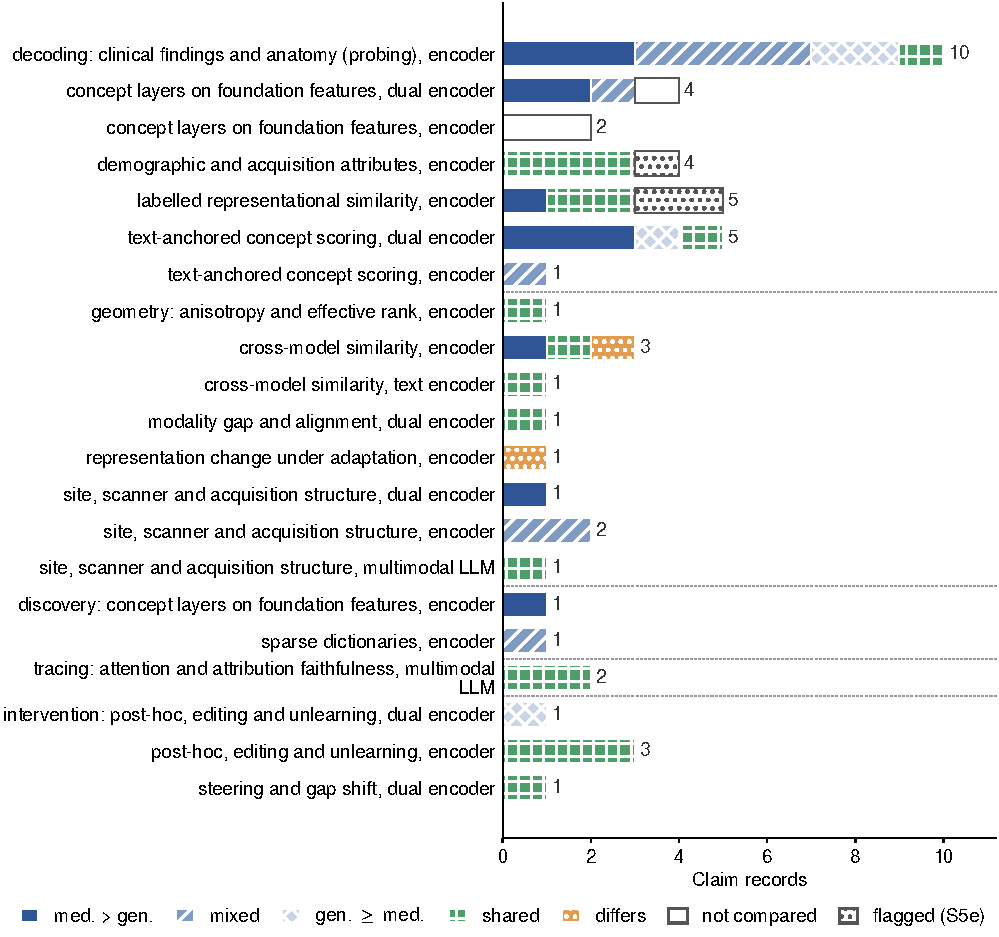
\includegraphics[width=\linewidth]{fig7_mvg.pdf}
\caption{The \Nmvgrec{} same-data medical-versus-general comparisons, by stratum: the property tested
(coding-sheet family and sub-group) crossed with the model object compared (from the locus), split by the
coded outcome. \emph{med.\ $>$ gen.}: the medical model shows more of the tested property or performs better;
\emph{gen.\ $\geq$ med.}: the general model matches or exceeds it; \emph{mixed}: the result differs across
tasks or models; \emph{shared}: the property is present in both kinds of model; \emph{differs}: it is present
in one kind only; \emph{not compared}: the general model is measured only on a quantity other than the coded
property, such as zero-shot accuracy. The properties are not commensurable and the strata are not summed;
F10 and F11 in \S7 of the article inventory these records without an aggregate direction. Records
whose study carries a critical defect touching their claim appear as \emph{defect-touched}, the same
defect screen the article uses. Most strata hold one to five records,
which is why no pooled effect is reported (supplement S6b). The three ordered outcomes use the
navy-to-pale ramp of Fig.~7 of the article; green and orange mark the two nominal outcomes and never an
ordered level.}
\label{fig:mvg}
\end{figure*}
\FloatBarrier

\section*{The validity-test rubric and the defect screen}
The full validity-test rubric (Table~S11): for each of the \Vnclasses{} classes, what the design already
supports without it, and what the class adds and does not add; and the defect screen (Table~S12), the five
recorded result-invalidating defect kinds behind the flagged records, which the article marks rather than
removes (the screen as a sensitivity is in S6). The article's Table~\ref{tab:vcov} carries the one-clause
version with the record counts.
\renewcommand{\thetable}{S11}\begin{sidewaystable*}[p]
\centering\footnotesize\setlength\tabcolsep{4pt}\renewcommand{\arraystretch}{1.05}
\caption{What each validity test licenses, and what it does not. No test is a prerequisite for the base reading of its family: held-out performance above the study-stated reference already licenses column~2, and each class licenses the strictly stronger statement in column~3, which also states the reading the class does \emph{not} support. A row of \S\ref{sec:findings} lacking a class is therefore \emph{narrower}, not uncontrolled, and the classes are never summed. How many records report each class, with a one-clause version of this rubric, is Table~\ref{tab:vcov} of the article. Intervention specificity applies when the operation targets a specific direction, feature, unit or token, named or not; distributional corrections, editing and unlearning are outside it and are not counted as failures, the comparison each needs being stated in Table~\ref{tab:families}.}
\label{tab:rubric}
\begin{tabular}{@{}L{3.0cm}L{3.6cm}L{10.5cm}L{3.6cm}@{}}
\toprule
Validity-test class \emph{(designs it applies to)} & What the design already supports without it & What the class adds, and what it does not & Tests coded under it (records) \\
\midrule
Sample-level permutation control \emph{(fitted probes and concept vectors; intrinsic designs)} & the fitted pipeline returns the reported value on these data & the value exceeds what the \emph{whole fitted procedure} returns when the labels are permuted across examples and it is refitted, which bounds what it can extract from labels carrying no information. It does \emph{not} hold the structure of the task fixed, which is what a randomized control task adds, nor show that the readout tracks the target rather than a correlated attribute & sample-level label permutation with refit (3) \\
Reference-distribution calibration \emph{(all decoding designs; intrinsic designs; structural and geometric)} & the statistic takes the reported value on these data & the value is placed on a scale --- an analytical chance level, a hypergeometric null, or a distribution over unrelated pairs --- so it can be read as high or low rather than as a bare number. It calibrates the statistic and does \emph{not} bound what the fitting procedure could have extracted & chance, shuffled or null reference (4) \\
Randomized control task \emph{(fitted probes and concept vectors; intrinsic designs)} & the measurement returns the reported value on these data & the readout is selective rather than expressive: a control task in the sense of Hewitt and Liang assigns each input \emph{type} a fixed random label, preserving the structure of the task while destroying its content, refits the same probe, and reports selectivity as the gap. It differs from a sample-level permutation, which reassigns labels per example and is reported in \Vperm{} records; no record reports a control task proper. The construction needs repeated input \emph{types}, which medical images seldom have and which is not coded per record, so the denominator is an \emph{upper bound on applicability} rather than a count of omitted safeguards (\S\ref{sec:future}) & none reported \\
Matched-object control \emph{(all decoding designs; intrinsic designs)} & the measurement returns the reported value on these data & the reported quantity follows the fitted object rather than any object of that size --- a direction matched in rank to the fitted one, an equal-size random unit set, a no-encoder baseline. It does \emph{not} say what the readout tracks, which is the control task above & matched-object control (1) \\
Planted ground truth \emph{(all decoding designs; intrinsic designs)} & the operator returns some value on real data, whose correctness is unknown & the operator returns the known answer on a condition built to have one (an injected bias, a planted encoder, a graded confound mixture). This validates the \emph{instrument}; it carries to the real-data claim only under the assumption that the planted condition resembles it & planted ground truth (4) \\
Learned-representation attribution \emph{(all decoding designs; intrinsic designs; geometry; tracing)} & the trained model's representation affords the reported value & the structure is a product of training rather than of the architecture and the input statistics, since an untrained or randomised encoder of the same shape does not afford it & randomly initialised encoder (4), embedding-randomisation control (1) \\
Comparison model \emph{(structural and geometric)} & the statistic takes the reported value on this model & the value differs from another model's under the same measurement --- a general encoder, a supervised classifier or a conventional feature pipeline. It does \emph{not} establish that the value is unusual in absolute terms; that needs a null & comparison model (16) \\
Semantic validation \emph{(feature decomposition and discovery)} & a unit exists in the fitted decomposition and its top activations can be displayed & the unit corresponds to the concept it is named for, as judged by clinicians or by structured labels, rather than by the analyst's reading of its exemplars & label validation (10), clinician validation (7), clinician and label validation (1) \\
Input-space corroboration \emph{(attribution, localisation and tracing)} & the map or component covaries with the output & the output depends on the region or input property the map highlights, since occluding, deleting, flipping or counterfactually altering it moves the output. It does \emph{not} establish that any particular internal component carries the behaviour: the intervention is on the input, not on the representation & perturbation confirmation (4), counterfactual confirmation (1), occlusion confirmation (1) \\
Internal-component perturbation \emph{(tracing; intrinsic designs)} & the map or component covaries with the output & the output changes when the internal component is perturbed --- masked, patched or replaced --- rather than when the input is. The credited designs are perturbations, not identified on-manifold interventions: neither on-manifold editing nor magnitude control is coded, so the class licenses causal implication under those assumptions rather than establishing them. Specificity to \emph{that} component needs a matched control & activation patching or masking (1), intervention on the concept layer (1) \\
Intervention specificity \emph{(representation intervention, targeted operations only)} & the edit changes the output & the change follows the targeted direction, feature, unit or token rather than the act of perturbing a representation of that size & matched control (3) \\
\bottomrule
\end{tabular}
\end{sidewaystable*}

\renewcommand{\thetable}{S12}\begin{table}[!t]
\centering\footnotesize\setlength\tabcolsep{3pt}\renewcommand{\arraystretch}{1.08}
\caption{The defect screen: the five recorded result-invalidating defect kinds behind the records that the article marks as flagged. A record is flagged when its study carries one of these defects \emph{and} the defect touches that record's own claim (or its applicability is uncertain); a defect concerning another record of the same study leaves this one unmarked. The screen is the review's own rule, fixed before the findings were assembled; it is not a risk-of-bias instrument, and the article counts every record, flagged or not, reporting in S6 what setting the flagged records aside changes. Per-record judgements are listed in supplement S5e.}
\label{tab:defects}
\begin{tabular}{@{}L{1.9cm}L{2.4cm}L{2.0cm}r@{}}
\toprule
Defect & What it is & Why it invalidates the quantity & Rec. \\
\midrule
resubstitution & a probe or dictionary is fitted and scored on the same data & the reported quantity is an optimistically biased estimate of held-out performance, by an amount the data do not reveal & 8 \\
leakage across split units & a slide, patient or site appears on both sides of the split & the score is a within-unit score reported as an across-unit one & 7 \\
circular estimation & the quantity is estimated from a dependence the design created & the estimate is a property of the pipeline, not of the representation & 6 \\
selection on the reported metric & the configuration is chosen on the number reported & the number is a maximum over choices, reported as a single draw & 2 \\
single-case fitting & the fitting block is one case & nothing separates the case from the property & 1 \\
\midrule
Total & records with a recorded defect of these kinds & 19 touched, 1 uncertain, 4 left in & 24 \\
\bottomrule
\end{tabular}
\end{table}

\FloatBarrier

\section*{Design of the dictionary-learning studies}
The design of every dictionary-learning study in the corpus (Table~S13), extracted from the full texts: the
model and locus, the token and layer decomposed, the method and width, how features were named, how the
names were validated, whether reproducibility was checked, and the reconstruction quality reported.
\renewcommand{\thetable}{S13}\begin{sidewaystable*}[p]
\centering\scriptsize\setlength\tabcolsep{3.5pt}\renewcommand{\arraystretch}{0.92}
\caption{Design of the core dictionary-learning studies (supplementary Table~S13; the factorisation, dissection and activation-atlas studies are not dictionaries and are omitted), extracted from the full texts. Activations: model, token type and layer the dictionary is trained on. Method: ReLU/L1 = standard sparse autoencoder; TopK/BatchTopK, Matryoshka and gated variants as named by the authors. Width: expansion factor (dictionary size). Naming: how features are named. Validation: how names or features are validated (expert = clinician reading of the features or their names, with the number of readers where stated; label agreement = agreement with structured labels or regions; LLM judge = an independent language or vision--language model); the \Nsaeval{} of the \Nsae{} studies carry expert or label validation and are what finding F7 selects (\S\ref{sec:findings}); the remaining six (LLM judge only, downstream only, causal check only, planned, or a reader study of generated reports) carry none. The table lists every dictionary study in the corpus, so it has as many rows as there are dictionary studies. Stability: any reproducibility reported (seeds, cohorts, training sets, architectures). Recon.: reconstruction quality (EV/FVE = explained variance; $R^2$; cosine). n.r. = not reported.}
\label{tab:saedesign}
\begin{tabular}{@{}L{2.80cm}L{3.85cm}L{2.51cm}L{1.73cm}L{2.26cm}L{2.93cm}L{1.73cm}L{1.46cm}@{}}
\toprule
Study & Activations & Method & Width & Naming & Validation & Stability & Recon. \\
\midrule
\cite{le2024learning} & PLUTO (path.); CLS; output & ReLU/L1 & 8$\times$ (1--32 swept) & manual + label match & label agreement ($\rho$ 0.70) & cross-set match ($\rho$ 0.96) & n.r. \\
\cite{abdulaal2024an} & RAD-DINO (CXR); CLS; output & gated SAE & 64$\times$ (49k) & auto-LLM from reports & reader study of generated reports (1 radiologist) + RadFact; features not directly validated & n.r. & EV 84\% \\
\cite{renzulli2025medsae} & MedCLIP (CXR); pooled; last & ReLU/L1 & 16$\times$ (8k) & auto-LLM (MedGemma) & LLM judge + label agreement & n.r. & FVE 0.98 \\
\cite{tang2025cxrlanic} & BiomedCLIP classifier (CXR); pooled & TopK transcoder ($\times$100) & 15k each & auto-LLM (planned) & planned only & n.r. & n.r. \\
\cite{nakka2025mammosae} & Mammo-CLIP (mammo.); patch; final & ReLU/L1 & 8$\times$ (16k) & label match & label agreement (mAP); AUC drop $<$2\% & n.r. & downstream \\
\cite{dasdelen2025cytosae} & DinoBloom (cytology); patch+CLS; L11 & ReLU/L1 & 64$\times$ (49k) & manual (1 expert) & expert (n=1) & 3 seeds & n.r. \\
\cite{sun2025prototypebased} & CONCH (path.); tile; output & ReLU/L1 & 4$\times$ (2k) & manual (pathologists) & expert (75--86\% monosemantic) & n.r. & n.r. \\
\cite{bouzid2025insights} & MAIRA-2 LLM; residual token; L15/32 & Matryoshka + BatchTopK & 4$\times$ (16k) & auto-LLM (GPT-4o) & LLM judge & n.r. & n.r. \\
\cite{kim2026dissecting} & Virchow2 (path.); tile; output & TopK ($k$=30) & 32$\times$ (41k) & manual (2 pathologists) & expert (2) + downstream & n.r. & EV $>$0.8 \\
\cite{wesp2026sparse} & BiomedParse, DINOv3 (CT/MRI); pooled & Matryoshka + BatchTopK & nested 128--8k & auto-LLM (MedGemma) & LLM judge + label agreement & n.r. & $R^2$ 0.89--0.94 \\
\cite{nerrise2026geosae} & BrainIAC (MRI); CLS; all 12 layers & TopK ($k$=16) + manifold & 2$\times$ (1.5k) & label match (partial corr.) & label agreement + downstream & cross-cohort & EV $>$99\% \\
\cite{yan2026a} & PanDerm (derm.); pooled; output & ReLU/L1 & 8$\times$ & text matching & label agreement (P@50 0.94) & n.r. & n.r. \\
\cite{nooralahzadeh2026universal} & RadVLM LLM; residual token; 10 layers & TopK ($K$=64) & 8$\times$ (33k) & none (causal selection) & downstream only & cross-arch.\ overlap & cos.\ 0.97--0.99 \\
\cite{sadanandan2026mechanistically} & MedGemma LLM; residual token; L17 & Gemma Scope 2 (reused) & n.r. & manual (1 feature) & causal patching & n.r. & $R^2$ 0.997 \\
\cite{haque2026medconcept} & Merlin (CT); volume emb.; output & ReLU/L1 & 2$\times$ & text matching (UMLS) & LLM judge & n.r. & n.r. \\
\cite{zhao2026compositional} & UNI (path.); tile emb.; output & ReLU + L0 target & 64$\times$ (66k) & manual (pathologists) & expert (several) + CyCIF & partial (feature scores) & L2 loss reported \\
\cite{bisson2026unsupervised} & CONCH v1.5 (path.); tile emb.; output & L1 (activation n.r.) & 1$\times$ (768) & manual (3 pathologists) & expert (3) + downstream & n.r. & n.r. \\
\cite{redlich2026explainable} & Virchow2 (path.); tile emb.; output & TopK ($K$=8) & 6$\times$ (7.7k) & manual (3 neuropathologists) & expert (3; 21/24 patterns) & partial (activation diff.) & n.r. \\
\bottomrule
\end{tabular}
\end{sidewaystable*}

\FloatBarrier

\section*{Sub-types of the decoding and intervention families}
The sub-types that article Table~\ref{tab:families} folds into their families (Table~S14): zero-shot
scoring, concept activation vectors and labelled similarity for decoding; post-hoc transformation of stored
embeddings and parameter editing or unlearning for intervention.
\renewcommand{\thetable}{S14}\begin{table*}[!tbp]
\centering\footnotesize\setlength\tabcolsep{4pt}\renewcommand{\arraystretch}{1.1}
\caption{Sub-types of the decoding and intervention families, as in article Table~\ref{tab:families}: the claim each licenses on its own, the test that licenses a stronger reading, and where this corpus stops. Zero-shot scoring, concept activation vectors and labelled similarity are decoding designs with no fitted decoder, a gradient-associated direction and a correspondence of distances respectively; post-hoc transformation of stored embeddings and parameter editing or unlearning are intervention sub-types with estimands of their own (\S\ref{sec:intervention}).}
\label{tab:familiessub}
\begin{tabular}{@{}L{3.0cm}L{4.6cm}L{3.6cm}L{4.1cm}@{}}
\toprule
Sub-type & Claim licensed on its own & Stronger reading needs & Where this corpus stops \\
\midrule
\multicolumn{4}{@{}l}{\emph{Supervised concept mapping and decodability}} \\
\emph{zero-shot scoring} & $c$ recoverable by a fixed scorer ($\cos(z_v,z_t)$), once validated on held-out labels & prompt-set sensitivity; held-out validation & expert-validated concepts a minority; prompt sensitivity unreported \\
\emph{concept activation vectors} & logit gradient-associated with a fitted direction (TCAV $S_{c,k}$), not recoverability & random-direction null; refit on shuffled labels & refit on shuffled labels: no record \\
\emph{labelled similarity} & representation and concept distances correspond (RSA); no held-out value & permutation null over the labelled sets & permutation null: one record of five \\
\addlinespace[3pt]
\multicolumn{4}{@{}l}{\emph{Representation intervention and control}} \\
\emph{post-hoc transformation of stored embeddings} & changes what a refitted readout can do, not the model's computation & sham or alternative transformation; unrelated-attribute control & downstream evaluation only; no sham transformation \\
\emph{parameter editing and unlearning} & behaviour changes as specified; no mediator unless measured & locality and retain-set checks; a measured mediator & no representation-level mediator identified \\
\bottomrule
\end{tabular}
\end{table*}

% flush every table before the reference list: tables must not interleave with it
\FloatBarrier
\clearpage
\bibliographystyle{elsarticle-num-np}
\bibliography{refs,refs_extra}
\end{document}
